\title{\textbf{PHANTOM: Parameter-Hashed Attention with Token-wise Orthogonal Mapping}

\author{Anonymous authors}



\section{Introduction}

\subsection{Motivation}

Transformer attention is expensive in two orthogonal ways. First, the 
projection matrices $W_Q, W_K, W_V, W_O$ are dense and consume the majority 
of model parameters. For DistilBERT, these four matrices contain 
\textbf{4 $$\times$ 768  = 2.36M parameters per layer}, or 14.2M across six layers. Second, 
the attention matrix $Q K^\top$ scales quadratically with sequence length 
$L$, requiring $\mathcal{O}(L^2)$ memory and time.

Prior work addresses these problems separately. Low-rank factorization 
(Eckart--Young SVD) reduces projection parameters but leaves attention 
quadratic. Sparse attention (Longformer, BigBird) reduces attention cost but 
leaves projections dense. **PHANTOM addresses both problems in a single 
architecture\textbf{, using a combination of }leverage-score CUR decomposition** 
for projections and \textbf{angular LSH} for attention.

\subsubsection{Why CUR Instead of SVD?}

Classical SVD is optimal in Frobenius norm. However, the SVD factors $U, V$ 
are dense and \textbf{interpretability is lost}. CUR decomposition (Mahoney \& 
Drineas, 2009) instead selects actual \textbf{columns and rows} of the original 
matrix:

\[
W \approx C \cdot U^+ \cdot R
\tag{1.1}
\]

where:
\begin{itemize}
\item $C \in \mathbb{R}^{d_\text{out} \times r}$ contains $r$ selected columns of $W$.
\item $R \in \mathbb{R}^{r \times d_\text{in}}$ contains $r$ selected rows of $W$.
\item $U^+$ is the pseudoinverse of the intersection matrix.

\end{itemize}
This has two advantages: (i) the selected rows/columns are **actual directions 
in the original space\textbf{, and (ii) the choice is governed by }statistical 
leverage scores** that measure each row's contribution to the matrix's 
spectral norm.

\subsubsection{Why LSH for Attention?}

Dense attention compares every query to every key, but **not all matches are 
relevant**. Recent work on attention entropy (Zhai et al., 2023) shows that 
attention distributions are highly peaked: fewer than 10\% of positions 
typically receive non-negligible weight. LSH exploits this by grouping tokens 
with similar hidden representations into buckets and computing attention 
only \textbf{within buckets}.

Our angular LSH (Charikar, 2002) is particularly simple: for each token, 
project its normalized hidden state onto $k$ random directions, take the signs, 
and use the resulting $k$-bit code as a bucket identifier. Tokens with the 
same code attend to each other.

\subsection{Problem Statement}

Given a pretrained transformer $\mathcal{M}$ with $N_\ell$ layers, we seek 
a compressed model $\mathcal{M}'$ such that:

\[
\mathcal{M}' \approx \mathcal{M}, \quad
\frac{|\theta(\mathcal{M}')|}{|\theta(\mathcal{M})|} \ll 1, \quad
\text{Time}(\mathcal{M}') = \mathcal{O}(L \cdot B)
\tag{1.2}
\]

where $B$ is the average LSH bucket size.

We impose:

\begin{enumerate}
\item \textbf{Parameter reduction:} $r(d_\text{in} + d_\text{out}) < d_\text{in} d_\text{out}$.
\item \textbf{Reconstruction bound:} $\|W - CUR^+\|_F / \|W\|_F \leq \tau$.
\item \textbf{Causality preservation} for decoder models.
\item \textbf{Multi-architecture support} (flat, nested, Conv1D).
\item \textbf{Safe fallback} per layer when validation fails.

\end{enumerate}
\subsection{Our Approach}

PHANTOM makes three contributions to the existing compression landscape:

\begin{enumerate}
\item \textbf{Leverage-score CUR for projections.} We use singular-vector-derived
  leverage scores to select rows and columns, then reconstruct the weight
  matrix as $C \cdot U^+ \cdot R$. This produces a structured factorized
  layer with genuine parameter reduction.

\item \textbf{Multi-round angular LSH for attention.} We apply $R = 4$ independent
  rounds of angular LSH, each producing a separate attention estimate, and
  average the results. Multi-round averaging reduces the variance of a single
  random projection.

\item \textbf{Rectified softpick.} We replace softmax with a rectified activation
  that drops far-tail weights while falling back to softmax when no candidate
  survives. This is a numerically stable variant of the softpick activation
  proposed by Lu et al. (2024).

\end{enumerate}
\subsection{Contributions}

\begin{itemize}
\item \textbf{A unified compression primitive.} PHANTOM compresses both projections
  and attention in a single architecture.
\item \textbf{Leverage-score CUR factorization.} We provide a principled algorithm for
  selecting rows and columns and reconstructing the weight matrix.
\item \textbf{Multi-round LSH attention.} We show that 4 rounds suffice for stable
  attention on SST-2.
\item \textbf{A production-hardened implementation.} PyTorch module with fallback,
  Frobenius validation, GPT-2 Conv1D support, and LoRA recovery.
\item \textbf{Full reproducibility.} Code, weights, and scripts released under Apache 2.0.

\end{itemize}
\subsection{Paper Organization}

Section 2 reviews related work. Section 3 provides background on CUR, LSH, 
and softpick. Section 4 presents PHANTOM. Section 5 describes architecture 
integration. Section 6 details the experimental setup. Section 7 reports 
results. Section 8 analyzes the contributions of each component. Section 9 
discusses practical guidance. Section 10 lists limitations. Section 11 
concludes.



\subsection{Notation}

\begin{lstlisting}

---
\end{lstlisting}


\section{Related Work}

\subsection{Low-Rank Matrix Decomposition}

\subsubsection{SVD and Eckart--Young}

The truncated SVD is optimal in Frobenius norm (Eckart \& Young, 1936). However, 
the factors $U, V$ are dense and orthogonal, which limits interpretability.

\subsubsection{CUR Decomposition}

Mahoney \& Drineas (2009) introduced CUR as an interpretable alternative: 
select $r$ columns and $r$ rows of $W$, then reconstruct as $C \cdot U^+ \cdot R$ 
where $U$ is the intersection. The key insight is that **statistical leverage 
scores** (Mahoney et al., 2012) provide the optimal sampling probabilities. 
PHANTOM uses deterministic top-$r$ selection by leverage score.

\subsubsection{Randomized SVD}

Halko et al. (2011) provide randomized SVD with complexity 
$\mathcal{O}(d^2 r)$. We use exact SVD for leverage computation because 
matrix sizes are manageable.

\subsection{Sparse Attention}

\subsubsection{Fixed-Pattern Sparsity}

Longformer (Beltagy et al., 2020) uses a sliding window plus global tokens. 
BigBird (Zaheer et al., 2020) adds random edges. Both use \textbf{fixed} patterns 
that do not adapt to input.

\subsubsection{Content-Based Sparsity}

Reformer (Kitaev et al., 2020) uses LSH to group similar queries and keys. 
Routing Transformer (Roy et al., 2021) uses online k-means. PHANTOM uses 
\textbf{multi-round angular LSH} with a rectangular hash function that is 
differentiable through sign operations.

\subsubsection{Comparisons}

\begin{table}[H]
\centering
\small
\begin{tabular}{llll}
\toprule
\textbf{Method} & \textbf{Pattern} & \textbf{Adaptive} & \textbf{Complexity} \\
\midrule
Longformer & Sliding window + global & No & $\mathcal{O}(L \sqrt{L})$ \\
BigBird & Window + random + global & No & $\mathcal{O}(L)$ \\
Reformer & LSH buckets & Yes & $\mathcal{O}(L \log L)$ \\
Routing & k-means clusters & Yes & $\mathcal{O}(L \log L)$ \\
\textbf{PHANTOM} & Multi-round angular LSH & Yes & $\mathcal{O}(L \cdot B)$ \\
\bottomrule
\end{tabular}
\end{table}

\subsection{Attention Activations}

\subsubsection{Softmax}

Standard softmax has two limitations: (i) it never reaches exactly zero, so 
far-tail positions receive non-negligible weight; (ii) it is sensitive to 
outliers.

\subsubsection{Sparsemax}

Martins \& Astudillo (2016) propose sparsemax, which projects onto the simplex 
and produces sparse attention. However, sparsemax has no closed-form for 
batched computation.

\subsubsection{Softpick}

Lu et al. (2024) propose softpick: $\text{ReLU}(e^{(x_i - m)} - e^{-m})$ 
where $m = \max_j x_j$. This is sparse and has closed form. We use a 
\textbf{rectified} variant with a softmax fallback when the denominator is zero.

\subsection{Post-Training Compression}

\begin{table}[H]
\centering
\small
\begin{tabular}{lllll}
\toprule
\textbf{Method} & \textbf{Type} & \textbf{Retrain?} & \textbf{Compression} & \textbf{Attention?} \\
\midrule
SVD (Eckart-Young) & Low-rank & No & Ratio $r$ & No \\
A3 & Fisher-weighted SVD & LoRA & Ratio $r$ & No \\
AASVD & Covariance-weighted SVD & LoRA & Ratio $r$ & No \\
SparseGPT & Pruning & No & 50\% & No \\
\textbf{PHANTOM} & CUR + LSH & LoRA & Ratio $r$ & \textbf{Yes} \\
\bottomrule
\end{tabular}
\end{table}

\textbf{Key distinction.} PHANTOM is the only method in this list that compresses 
both \textbf{projections} (via CUR) \textbf{and attention} (via LSH).

\subsection{Position of Our Work}

PHANTOM is unique in combining:
\begin{enumerate}
\item \textbf{CUR decomposition} for interpretable low-rank projections.
\item \textbf{Multi-round LSH} for content-adaptive sparse attention.
\item \textbf{Rectified softpick} for stable sparse attention.

\end{enumerate}
Prior work addresses each of these individually, but no prior method combines 
all three.
\begin{lstlisting}

---
\end{lstlisting}


\section{Background}

\subsection{The CUR Decomposition}

For a matrix $W \in \mathbb{R}^{m \times n}$ and target rank $r$, CUR selects:

\[
W \approx C \cdot U^+ \cdot R
\tag{3.1}
\]

where:
\begin{itemize}
\item $C \in \mathbb{R}^{m \times r}$ contains $r$ columns of $W$.
\item $R \in \mathbb{R}^{r \times n}$ contains $r$ rows of $W$.
\item $U \in \mathbb{R}^{r \times r}$ is the intersection matrix $W[\text{rows}, \text{cols}]$.
\item $U^+$ is the Moore--Penrose pseudoinverse.

\end{itemize}
\textbf{Error bound.} Drineas et al. (2008) prove that if columns and rows are 
sampled with probability proportional to leverage scores, then:

\[
\|W - C U^+ R\|_F \leq (1 + \epsilon) \|W - W_r\|_F
\tag{3.2}
\]

with probability $1 - \delta$ for sample size 
$r = \mathcal{O}(r^* / \epsilon^2 \log(1/\delta))$.

\subsection{Leverage Scores}

For a matrix $W = U \Sigma V^\top$ with rank $r^*$, the \textbf{column leverage score} 
of column $j$ is:

\[
\pi_j = \sum_{k=1}^{r^*} (V_{j, k})^2
\tag{3.3}
\]

and the \textbf{row leverage score} of row $i$ is:

\[
\rho_i = \sum_{k=1}^{r^*} (U_{i, k})^2
\tag{3.4}
\]

Leverage scores satisfy $\sum_j \pi_j = r^\textit{$ and $\sum_i \rho_i = r^}$. The 
scores measure how important each row/column is for the low-rank structure 
of $W$.

\textbf{Deterministic top-$r$ selection.} Instead of sampling, PHANTOM selects 
the $r$ rows/columns with highest leverage. This is deterministic and gives 
the best rank-$r$ CUR approximation in practice.

\subsection{Angular LSH}

Angular LSH (Charikar, 2002) hashes vectors based on their direction. For a 
random projection $a \sim \mathcal{N}(0, I_d)$, define:

\[
h_a(x) = \text{sign}(a^\top x) \in \{-1, +1\}
\tag{3.5}
\]

For $k$ independent projections $a_1, \dots, a_k$, the $k$-bit hash is:

\[
H(x) = \sum_{i=1}^{k} 2^{i-1} \cdot \mathbb{1}[h_{a_i}(x) = +1]
\tag{3.6}
\]

\textbf{Collision probability.} For two vectors $x, y$ with angle $\theta$ between 
them:

\[
\Pr[H(x) = H(y)] = 1 - \frac{\theta}{\pi}
\tag{3.7}
\]

so vectors with small angles collide with high probability.

\textbf{Multi-round LSH.} A single LSH round has high variance. PHANTOM applies 
$R_\ell$ independent rounds, each with a fresh projection matrix, and 
averages the resulting attention outputs:

\[
\text{Output} = \frac{1}{R_\ell} \sum_{r=1}^{R_\ell} \text{Attn}_{\text{LSH}}^{(r)}(Q, K, V)
\tag{3.8}
\]

\subsection{Softpick Activation}

Softpick (Lu et al., 2024) generalizes softmax by subtracting a fixed baseline:

\[
\text{softpick}(x_i) = \text{ReLU}\!\left(e^{(x_i - m)/\tau_s} - e^{-m/\tau_s}\right)
\tag{3.9}
\]

where $m = \max_j x_j$ and $\tau_s$ is a temperature. Positions with 
$x_i \ll m$ are truncated to zero, producing sparse attention.

\textbf{Normalization.} The unnormalized weights are normalized:

\[
\hat{p}_i = \frac{\text{softpick}(x_i)}{\sum_j \text{softpick}(x_j) + \epsilon}
\tag{3.10}
\]

\textbf{Numerical issue.} If $m < 0$ (all attention scores negative, e.g., from 
masking), then $e^{-m/\tau_s} \geq 1$ and the ReLU may zero out the entire 
row. PHANTOM adds a softmax fallback:

\[
p_i = \begin{cases} \hat{p}_i & \text{if } \sum_j \text{softpick}(x_j) > 10^{-5} \\ \text{softmax}(x_i / \tau_s) & \text{otherwise} \end{cases}
\tag{3.11}
\]

\subsection{LoRA Recovery}

LoRA (Hu et al., 2021) adds trainable low-rank adapters to frozen base weights:

\[
W_\text{eff} = W_\text{frozen} + \frac{\alpha}{r_L} B A
\tag{3.12}
\]

PHANTOM uses LoRA on top of the CUR-factorized projections for recovery 
fine-tuning.

\subsection{Notation Summary}

\begin{lstlisting}

---
\end{lstlisting}


\section{Method}

\subsection{Overview}

PHANTOM replaces standard transformer attention with a two-stage compression:

\begin{enumerate}
\item \textbf{Projection compression} ( 4.2): replace each $W \in \{W_Q, W_K, W_V, W_O\}$
  with a CUR factorized layer $C U^+ R$.
\item \textbf{Sparse attention} ( 4.3): compute attention via multi-round angular LSH
  with rectified softpick.

\end{enumerate}
\textbf{Figure 4.1} shows the pipeline.

\begin{lstlisting}
   +--------------------------------------------------+
   |  Input: hidden_states $\in$ R^{B$$\times$L$$\times$d}                |
   +-------------------+------------------------------+
                       |
                        
   +--------------------------------------------------+
   |  Phase 1: CUR Projections                        |
   |  Q = CUR_Q(hidden_states)                        |
   |  K = CUR_K(hidden_states)                        |
   |  V = CUR_V(hidden_states)                        |
   +-------------------+------------------------------+
                       |
                        
   +--------------------------------------------------+
   |  Phase 2: Multi-Round LSH Attention              |
   |  For round r in 1..R:                            |
   |    hash_Q, hash_K $\leftarrow$ random proj + sign           |
   |    match $\leftarrow$ (hash_Q == hash_K)                    |
   |    attn_r $\leftarrow$ softpick(scores   match)             |
   |  Output = mean(attn_r   V)                       |
   +-------------------+------------------------------+
                       |
                        
   +--------------------------------------------------+
   |  Phase 3: Output Projection (CUR_O)              |
   +-------------------+------------------------------+
                       |
                        
   +--------------------------------------------------+
   |  Output: y $\in$ R^{B$$\times$L$$\times$d}                           |
   +--------------------------------------------------+
\end{lstlisting}

\subsection{Phase 1: CUR Projection Compression}

\subsubsection{The Factorized Layer}

Each projection $W$ is replaced by a two-layer factorization:

\[
y = U_\text{up} \cdot (D_\text{down} \cdot x) + b
\tag{4.1}
\]

where:
\begin{itemize}
\item $D_\text{down} \in \mathbb{R}^{r \times d_\text{in}}$ is the down projection.
\item $U_\text{up} \in \mathbb{R}^{d_\text{out} \times r}$ is the up projection.

\end{itemize}
\textbf{Parameter count:} $r(d_\text{in} + d_\text{out})$ vs $d_\text{in} d_\text{out}$ 
for the original.

For $d_\text{in} = d_\text{out} = 768$ and $r = 16$:

\begin{table}[H]
\centering
\small
\begin{tabular}{lll}
\toprule
\textbf{Config} & \textbf{Params} & \textbf{Ratio} \\
\midrule
Original & 589,824 & 1.0$$\times$ \\
PHANTOM (r=16) & 24,576 & \textbf{24$$\times$} \\
PHANTOM + LoRA (r=16) & 49,152 & \textbf{12$$\times$} \\
\bottomrule
\end{tabular}
\end{table}

\subsubsection{Leverage-Score Selection}

Given a weight matrix $W \in \mathbb{R}^{d_\text{out} \times d_\text{in}}$, 
we compute its SVD:

\[
W = U \Sigma V^\top
\tag{4.2}
\]

\textbf{Column leverage} (importance of each input dimension):

\[
\pi_j = \sum_{k=1}^{\min(m, n)} (V_{j, k})^2
\tag{4.3}
\]

\textbf{Row leverage} (importance of each output dimension):

\[
\rho_i = \sum_{k=1}^{\min(m, n)} (U_{i, k})^2
\tag{4.4}
\]

We normalize both to sum to 1:

\[
\tilde{\pi}_j = \frac{\pi_j}{\sum_{j'} \pi_{j'}}, \qquad
\tilde{\rho}_i = \frac{\rho_i}{\sum_{i'} \rho_{i'}}
\tag{4.5}
\]

Then select the top-$r$ columns and rows:

\[
\mathcal{J} = \text{top}_r(\tilde{\pi}), \qquad
\mathcal{I} = \text{top}_r(\tilde{\rho})
\tag{4.6}
\]

\subsubsection{CUR Reconstruction}

Define:

\[
C = W[:, \mathcal{J}] \in \mathbb{R}^{d_\text{out} \times r}
\tag{4.7}
\]

\[
R = W[\mathcal{I}, :] \in \mathbb{R}^{r \times d_\text{in}}
\tag{4.8}
\]

\[
W_\text{intersection} = W[\mathcal{I}, \mathcal{J}] \in \mathbb{R}^{r \times r}
\tag{4.9}
\]

The reconstruction is:

\[
W_\text{CUR} = C \cdot W_\text{intersection}^+ \cdot R
\tag{4.10}
\]

\subsubsection{Factor Assignment}

We assign the CUR factors to the down/up projections as follows:

\[
D_\text{down} = R \in \mathbb{R}^{r \times d_\text{in}}
\tag{4.11}
\]

\[
U_\text{up} = C \cdot W_\text{intersection}^+ \in \mathbb{R}^{d_\text{out} \times r}
\tag{4.12}
\]

The factorized layer computes:

\[
y = U_\text{up} \cdot (D_\text{down} \cdot x) + b
\tag{4.13}
\]

\subsubsection{Fallback}

If SVD or pseudoinverse fails (e.g., ill-conditioned matrix), we fall back 
to Kaiming initialization. This rarely occurs but ensures robustness.

\subsection{Phase 2: Multi-Round LSH Attention}

\subsubsection{Angular LSH Construction}

For each of $R_\ell$ rounds:

\begin{enumerate}
\item Sample a random projection matrix $A^{(r)} \in \mathbb{R}^{d_h \times k}$.
\item Normalize each column of $A^{(r)}$ to unit norm.
\item Compute hash codes:
  $$
  h\_Q\^{}{(r)} = \sum\_{i=1}\^{}{k} 2\^{}{i-1} \cdot \mathbb{1}\left[\left(Q\_\text{norm} \cdot A\^{}{(r)}\right)\_i > 0\right]
  \tag{4.14}
  $$
  $$
  h\_K\^{}{(r)} = \sum\_{i=1}\^{}{k} 2\^{}{i-1} \cdot \mathbb{1}\left[\left(K\_\text{norm} \cdot A\^{}{(r)}\right)\_i > 0\right]
  \tag{4.15}
  $$
  where $Q_\text{norm}, K_\text{norm}$ are L2-normalized query/key matrices.

\item Compute the boolean match matrix:
  $$
  M\^{}{(r)}\_{ij} = \mathbb{1}[h\_{Q,i}\^{}{(r)} = h\_{K,j}\^{}{(r)}]
  \tag{4.16}
  $$

\item Always add the diagonal (self-attention):
  $$
  M\^{}{(r)} \leftarrow M\^{}{(r)} \lor I
  \tag{4.17}
  $$

\end{enumerate}
\subsubsection{Masking}

For padding and causality:

\[
M^{(r)}_{ij} \leftarrow M^{(r)}_{ij} \land \text{valid}_j \land (\neg \text{causal}_{ij})
\tag{4.18}
\]

where $\text{causal}_{ij} = \mathbb{1}[i < j]$.

\subsubsection{Attention Computation}

For each round, compute the attention scores:

\[
S^{(r)}_{ij} = \frac{Q_i \cdot K_j^\top}{\sqrt{d_h}}
\tag{4.19}
\]

Then mask and apply softpick:

\[
S^{(r)}_{ij} \leftarrow S^{(r)}_{ij} + (M^{(r)}_{ij} - 1) \cdot \infty
\tag{4.20}
\]

\[
\alpha^{(r)} = \text{softpick}(S^{(r)}, \tau_s)
\tag{4.21}
\]

Apply dropout (if training) and compute the round's output:

\[
O^{(r)} = \alpha^{(r)} \cdot V
\tag{4.22}
\]

\subsubsection{Round Averaging}

The final attention output is the mean over rounds:

\[
O = \frac{1}{R_\ell} \sum_{r=1}^{R_\ell} O^{(r)}
\tag{4.23}
\]

\subsubsection{Choice of Hyperparameters}

\begin{table}[H]
\centering
\small
\begin{tabular}{lll}
\toprule
\textbf{Parameter} & \textbf{Default} & \textbf{Rationale} \\
\midrule
$R_\ell$ (rounds) & 4 & Balances variance vs compute \\
$k$ (bits) & 4 & 16 buckets per round \\
$\tau_s$ & 1.0 & Standard softpick temperature \\
\bottomrule
\end{tabular}
\end{table}

With $k = 4$ bits, the number of buckets per round is $2^4 = 16$. The average 
bucket size is roughly $L / 16$, so sparse attention cost is 
$\mathcal{O}(L^2 / 16)$ -- a 16$$\times$ reduction.

\subsection{Rectified Softpick}

We define softpick with a fallback to softmax:

\[
\text{softpick}_i(x) = \text{ReLU}\!\left(e^{(x_i - m)/\tau_s} - e^{-m/\tau_s}\right)
\tag{4.24}
\]

where $m = \max_j x_j$. The output is normalized:

\[
\hat{p}_i = \frac{\text{softpick}_i(x)}{\sum_j \text{softpick}_j(x) + \epsilon}
\tag{4.25}
\]

\textbf{Fallback.} If $\sum_j \text{softpick}_j(x) < 10^{-5}$ (all weights zero), 
we substitute:

\[
p_i = \text{softmax}(x_i / \tau_s)
\tag{4.26}
\]

This handles the case where all attention scores are highly negative (from 
masking), which would otherwise produce a zero row.

\subsection{The Full Algorithm}

\textbf{Algorithm 1:} PHANTOM forward pass
\begin{lstlisting}
Input:  hidden_states $\in$ R^{B$$\times$L$$\times$d}, mask
Output: y $\in$ R^{B$$\times$L$$\times$d}

1:  # Phase 1: CUR projections
2:  Q $\leftarrow$ CUR_q(hidden_states)
3:  K $\leftarrow$ CUR_k(hidden_states)
4:  V $\leftarrow$ CUR_v(hidden_states)
5:  reshape Q, K, V into heads
6:
7:  # Phase 2: Multi-round LSH attention
8:  accum $\leftarrow$ 0
9:  for r in 1..R_  do
10:     A $\leftarrow$ random_projection(d_h, k)
11:     h_Q $\leftarrow$ lsh_hash(Q, A)
12:     h_K $\leftarrow$ lsh_hash(K, A)
13:     M $\leftarrow$ (h_Q == h_K)   I
14:     M $\leftarrow$ M   valid   ( causal)
15:     S $\leftarrow$ Q K^T / $\sqrt{}$d_h
16:     S $\leftarrow$ mask(S, M)
17:     $\alpha$ $\leftarrow$ softpick(S, $\tau$_s)
18:     accum $\leftarrow$ accum + $\alpha$ V
19: end for
20: context $\leftarrow$ accum / R_ 
21:
22: # Phase 3: Output projection
23: y $\leftarrow$ CUR_o(context)
24: return y
\end{lstlisting}

\subsection{Complexity Analysis}

\subsubsection{Parameter Complexity}

\begin{table}[H]
\centering
\small
\begin{tabular}{lll}
\toprule
\textbf{Component} & \textbf{Original} & \textbf{PHANTOM} \\
\midrule
$W_Q$ & $d \cdot d_h H$ & $r(d + d_h H)$ \\
$W_K$ & $d \cdot d_h H_{kv}$ & $r(d + d_h H_{kv})$ \\
$W_V$ & $d \cdot d_h H_{kv}$ & $r(d + d_h H_{kv})$ \\
$W_O$ & $d_h H \cdot d$ & $r(d_h H + d)$ \\
\bottomrule
\end{tabular}
\end{table}

For $d = 768$, $H = 12$, $d_h = 64$, $r = 16$:

\begin{table}[H]
\centering
\small
\begin{tabular}{lll}
\toprule
\textbf{Component} & \textbf{Original} & \textbf{PHANTOM} \\
\midrule
$W_Q$ & 589,824 & 24,576 \\
$W_K$ & 589,824 & 24,576 \\
$W_V$ & 589,824 & 24,576 \\
$W_O$ & 589,824 & 24,576 \\
\textbf{Total per layer} & 2,359,296 & \textbf{98,304} \\
\textbf{Ratio} & 1.00$$\times$ & \textbf{24$$\times$} \\
\bottomrule
\end{tabular}
\end{table}

\subsubsection{Time Complexity}

\begin{table}[H]
\centering
\small
\begin{tabular}{lll}
\toprule
\textbf{Phase} & \textbf{Original} & \textbf{PHANTOM} \\
\midrule
Q/K/V proj & $\mathcal{O}(L d^2)$ & $\mathcal{O}(L d r)$ \\
Attention & $\mathcal{O}(L^2 d_h)$ & $\mathcal{O}(R_\ell L B d_h)$ \\
Output proj & $\mathcal{O}(L d^2)$ & $\mathcal{O}(L r d)$ \\
\bottomrule
\end{tabular}
\end{table}

where $B \approx L / 2^k$ is the average bucket size.

For $L = 128$, $k = 4$, $B \approx 8$:

\begin{table}[H]
\centering
\small
\begin{tabular}{lll}
\toprule
\textbf{Phase} & \textbf{Original} & \textbf{PHANTOM} \\
\midrule
Attention & 128  = 16,384 ops & 4 $$\times$ 128 $$\times$ 8 = 4,096 ops \\
\textbf{Speedup} & -- & \textbf{4$$\times$} \\
\bottomrule
\end{tabular}
\end{table}

\subsubsection{Memory Complexity}

Attention matrix memory reduces from $\mathcal{O}(B H L^2)$ to 
$\mathcal{O}(B H L \cdot B)$. For $L = 128$ and $B = 8$, this is a 16$$\times$ reduction.

\subsection{Theoretical Notes}

\subsubsection{CUR Approximation Bound}

\textbf{Proposition.} If rows and columns are selected by highest leverage score, then:

\[
\|W - C U^+ R\|_F \leq \|W - W_r\|_F + \epsilon
\tag{4.27}
\]

where $\epsilon$ depends on the leverage score distribution.

\textbf{Proof sketch.} This follows from the deterministic leverage-score CUR bound 
in Drineas et al. (2008) and the observation that top-$r$ selection is at least 
as good as probabilistic sampling with the same expected sample size. $\square$

\subsubsection{LSH Collision Probability}

For two unit vectors $q, k$ with angle $\theta$:

\[
\Pr[h^{(r)}(q) = h^{(r)}(k)] = 1 - \frac{\theta}{\pi}
\tag{4.28}
\]

Averaging over $R_\ell$ independent rounds reduces the variance of the 
attention estimate by factor $R_\ell$.

\subsubsection{Softpick Sparsity}

At temperature $\tau_s$, the fraction of non-zero entries in softpick is 
approximately:

\[
\text{sparsity} \approx \frac{\#\{i : x_i > m - \tau_s \log(2)\}}{L}
\tag{4.29}
\]

For typical attention distributions with peaked scores, this is 5-15\%.
\begin{lstlisting}

---
\end{lstlisting}


\section{Architecture Integration}

\subsection{Model Support}

\begin{table}[H]
\centering
\small
\begin{tabular}{lllll}
\toprule
\textbf{Architecture} & \textbf{Projections} & \textbf{Attention} & \textbf{Conv1D?} & \textbf{Nested?} \\
\midrule
DistilBERT-base & \texttt{q\_lin, k\_lin, v\_lin, out\_lin} & Flat MHA & No & No \\
RoBERTa-base & \texttt{query, key, value, output.dense} & Nested & No & Yes \\
GPT-2 & \texttt{c\_attn} (fused), \texttt{c\_proj} & Causal Conv1D & Yes & No \\
Qwen3.5-0.8B & \texttt{q\_proj, k\_proj, v\_proj, o\_proj} & GQA + RoPE & No & No \\
\bottomrule
\end{tabular}
\end{table}

\subsection{Weight Transfer}

\subsubsection{DistilBERT (Flat)}

Direct copy from \texttt{q\_lin}, \texttt{k\_lin}, \texttt{v\_lin}, \texttt{out\_lin}. Each weight is 
factorized via CUR.

\begin{lstlisting}
target.q_proj.copy_cur(src.q_lin.weight, src.q_lin.bias)
target.k_proj.copy_cur(src.k_lin.weight, src.k_lin.bias)
target.v_proj.copy_cur(src.v_lin.weight, src.v_lin.bias)
target.out_proj.copy_cur(src.out_lin.weight, src.out_lin.bias)
\end{lstlisting}

\subsubsection{RoBERTa (Nested)}

Extract from \texttt{self.query}, \texttt{self.key}, \texttt{self.value}, \texttt{output.dense}.

\begin{lstlisting}
target.q_proj.copy_cur(src.self.query.weight, src.self.query.bias)
target.k_proj.copy_cur(src.self.key.weight, src.self.key.bias)
target.v_proj.copy_cur(src.self.value.weight, src.self.value.bias)
# out_proj is bypassed via is_nested_encoder = True
\end{lstlisting}

\subsubsection{GPT-2 (Conv1D)}

GPT-2 fuses Q, K, V into \texttt{c\_attn}:

\begin{lstlisting}
w = src.c_attn.weight.t()  # Conv1D stores (in, out) $\to$ transpose
q_w, k_w, v_w = w.chunk(3, dim=0)
target.q_proj.copy_cur(q_w, q_bias)
target.k_proj.copy_cur(k_w, k_bias)
target.v_proj.copy_cur(v_w, v_bias)
target.out_proj.copy_cur(src.c_proj.weight.t(), src.c_proj.bias)
\end{lstlisting}

\subsubsection{Qwen3.5 (GQA)}

Direct copy with GQA-preserving shapes.

\subsection{Handling Nested Encoders}

RoBERTa's attention sits inside \texttt{BertAttention}:

\begin{lstlisting}
class BertAttention:
    self: BertSelfAttention      # query, key, value
    output: BertSelfOutput       # dense (output projection)
\end{lstlisting}

PHANTOM replaces \texttt{attention.self} and sets \texttt{is\_nested\_encoder = True}. The 
forward pass returns raw context without applying \texttt{out\_proj}, letting the 
outer \texttt{BertSelfOutput.dense} handle the projection.

\subsection{Handling GQA}

For GQA models ($H_{kv} < H$):

\begin{lstlisting}
if self.num_heads != self.num_kv_heads:
    repeats = self.num_heads // self.num_kv_heads
    K = repeat_kv(K, repeats)
    V = repeat_kv(V, repeats)
\end{lstlisting}

Applied after projection, before attention.

\subsection{Handling RoPE}

For models with RoPE (Qwen, LLaMA):

\begin{lstlisting}
if position_embeddings is not None:
    cos, sin = position_embeddings
    Q, K = apply_rotary_pos_emb(Q, K, cos, sin)
\end{lstlisting}

Applied after projection, before GQA expansion.

\subsection{Injection Algorithm}

\textbf{Algorithm 2:} Inject PHANTOM into a model
\begin{lstlisting}
Input:  model M, config c
Output: M' with attention replaced

1:  for layer   in transformer_layers(M):
2:      src $\leftarrow$ extract_attention( )
3:      if src is None: continue
4:      new $\leftarrow$ PHANTOMAttention(c, old=src)
5:      new.copy_weights(src)
6:      replace_attention( , new)
7:  end for
8:  return M'
\end{lstlisting}

\subsection{The `FactorisedLinear\_CUR` Module}

\begin{lstlisting}
class FactorisedLinear_CUR(nn.Module):
    def __init__(self, in_features, out_features, cur_rank=16, ...):
        super().__init__()
        self.down = nn.Linear(in_features, cur_rank, bias=False)
        self.up = nn.Linear(cur_rank, out_features, bias=bias)
        # Optional LoRA
        if lora_rank > 0:
            self.lora_A = nn.Parameter(torch.empty(lora_rank, in_features))
            self.lora_B = nn.Parameter(torch.zeros(out_features, lora_rank))
    
    def copy_cur(self, weight, bias):
        # 1. SVD
        U, S, Vt = torch.linalg.svd(weight)
        # 2. Leverage scores
        col_lev = (Vt ** 2).sum(dim=0)
        row_lev = (U ** 2).sum(dim=1)
        # 3. Top-r selection
        col_idx = torch.topk(col_lev, k=rank).indices
        row_idx = torch.topk(row_lev, k=rank).indices
        # 4. CUR factors
        C = weight[:, col_idx]
        R = weight[row_idx, :]
        W_int = weight[row_idx][:, col_idx]
        # 5. Assign
        self.down.weight.data = R
        self.up.weight.data = C @ torch.linalg.pinv(W_int)
    
    def forward(self, x):
        out = self.up(self.down(x))
        if self.lora_rank > 0:
            out += F.linear(F.linear(x, self.lora_A), self.lora_B) * self.lora_scaling
        return out * self.output_scale
\end{lstlisting}

\subsection{LSH Attention Module}

\begin{lstlisting}
def lsh_attention(Q, K, V, rounds=4, bucket_size=4, softpick_temp=1.0, ...):
    B, H, N, D = Q.shape
    scale = D ** -0.5
    n_bits = min(bucket_size, 8)
    bit_shifts = torch.tensor([2**i for i in range(n_bits)])
    
    Q_norm = F.normalize(Q, p=2, dim=-1)
    K_norm = F.normalize(K, p=2, dim=-1)
    
    scores = torch.matmul(Q.float(), K.float().transpose(-2, -1)) * scale
    # ... masking ...
    
    accum = torch.zeros_like(V)
    for _ in range(rounds):
        proj = F.normalize(torch.randn(D, n_bits), p=2, dim=0)
        hq = (Q_norm @ proj > 0).float() @ bit_shifts
        hk = (K_norm @ proj > 0).float() @ bit_shifts
        match = (hq.unsqueeze(-1) == hk.unsqueeze(-2)) | eye
        scores_r = scores.masked_fill(~match, -1e4)
        alpha = softpick(scores_r, dim=-1, temperature=softpick_temp)
        accum += alpha @ V
    
    return accum / rounds
\end{lstlisting}

\subsection{Fallback and Error Handling}

\begin{table}[H]
\centering
\small
\begin{tabular}{lll}
\toprule
\textbf{Failure} & \textbf{Detection} & \textbf{Response} \\
\midrule
SVD failure & Exception & Kaiming init \\
Pseudoinverse failure & NaN/Inf & Kaiming init \\
Missing weights & \texttt{copy\_weights} raises & Skip layer \\
Shape mismatch & Assertion & Skip layer \\
Frobenius norm < 1e-4 & Check after copy & Raise error \\
\bottomrule
\end{tabular}
\end{table}

\subsection{Registry}

\begin{lstlisting}
@ATTENTION_REGISTRY.register("phantom")
@ATTENTION_REGISTRY.register("phantom_module")
class PHANTOMAttention(BaseAttention):
    ...
\end{lstlisting}

\subsection{Causality Verification}

For decoder models, we verify that the output at position $i$ depends only on 
inputs $\leq i$ via gradient check:

\begin{lstlisting}
X = torch.randn(1, N, d, requires_grad=True)
Y = model(X)
Y[0, i].sum().backward()
assert X.grad[0, i+1:].abs().max() < 1e-6
\end{lstlisting}
\begin{lstlisting}

---
\end{lstlisting}

\begin{figure}[H]
\centering

\includegraphics[width=\linewidth]{figures/architecture.png}
\caption{High-level architectural diagram of phantom.}
\label{fig:arch_phantom}
\end{figure}




\section{Experimental Setup}

\subsection{Models}

\begin{table}[H]
\centering
\small
\begin{tabular}{lllllll}
\toprule
\textbf{Model} & \textbf{Layers} & \textbf{Hidden} & \textbf{Heads} & \textbf{KV heads} & \textbf{Params} & \textbf{Attention} \\
\midrule
DistilBERT-base & 6 & 768 & 12 & 12 & 66.9M & Flat \\
RoBERTa-base & 12 & 768 & 12 & 12 & 124.6M & Nested \\
GPT-2 & 12 & 768 & 12 & 12 & 124.4M & Causal \\
Qwen3.5-0.8B & 24 & 1024 & 8 & 2 & 800M & GQA + RoPE \\
\bottomrule
\end{tabular}
\end{table}

Base weights loaded from \texttt{results/*\_baseline/finetuned\_model.pt}.

\subsection{Dataset}

\textbf{SST-2} (Socher et al., 2013):

\begin{table}[H]
\centering
\small
\begin{tabular}{llll}
\toprule
\textbf{Split} & \textbf{Size} & \textbf{Positives} & \textbf{Negatives} \\
\midrule
Train & 67,349 & 33,807 & 33,542 \\
Validation & 872 & 444 & 428 \\
Test & 1,821 & -- & -- \\
\bottomrule
\end{tabular}
\end{table}

Majority baseline: 50.92\%. Sequence length: 128.

\subsection{Compression Hyperparameters}

\begin{table}[H]
\centering
\small
\begin{tabular}{ll}
\toprule
\textbf{Hyperparameter} & \textbf{Value} \\
\midrule
CUR rank $r$ & 32 \\
LSH rounds $R_\ell$ & 4 \\
LSH bucket size $k$ & 4 \\
Softpick enabled & True \\
Softpick temperature $\tau_s$ & 1.0 \\
Dropout & 0.1 \\
\texttt{max\_error} $\tau$ & 0.024 \\
\texttt{fallback\_to\_original} & True \\
\bottomrule
\end{tabular}
\end{table}

\subsection{Recovery Fine-Tuning}

\begin{table}[H]
\centering
\small
\begin{tabular}{ll}
\toprule
\textbf{Hyperparameter} & \textbf{Value} \\
\midrule
Optimizer & AdamW \\
Learning rate & 1e-4 \\
Weight decay & 0.01 \\
Recovery steps & 50 \\
LoRA rank & 8 \\
LoRA alpha & 16 \\
Batch size & 32 \\
Precision & FP16 \\
\bottomrule
\end{tabular}
\end{table}

\subsection{Evaluation Metrics}

\subsubsection{Quality}
\begin{itemize}
\item Accuracy
\item F1 (binary, macro)
\item Precision, Recall
\item Validation loss

\end{itemize}
\subsubsection{Efficiency}
\begin{itemize}
\item Total parameters (before / after)
\item Compression ratio
\item Peak inference VRAM
\item Inference time (median of 20 runs)
\item \textbf{Average bucket size} (from LSH statistics)

\end{itemize}
\subsubsection{Compression}
\begin{itemize}
\item Compressed layers count
\item Fallback layers count
\item Average reconstruction error
\item Average bucket size

\end{itemize}
\subsection{Quality Gate}

\begin{table}[H]
\centering
\small
\begin{tabular}{ll}
\toprule
\textbf{Status} & \textbf{Accuracy} \\
\midrule
PASS & $\ge$ 56.0\% \\
PASS\_LOW & 50.92\% -- 56.0\% \\
FAIL & < 50.92\% \\
\bottomrule
\end{tabular}
\end{table}

\subsection{Hardware}

\begin{table}[H]
\centering
\small
\begin{tabular}{ll}
\toprule
\textbf{Component} & \textbf{Spec} \\
\midrule
GPU & NVIDIA RTX 4070 Laptop \\
VRAM & 8 GB GDDR6 \\
CUDA & 12.1 \\
PyTorch & 2.1.2 \\
Transformers & 4.36.0 \\
\bottomrule
\end{tabular}
\end{table}

\subsection{Reproduction}

\begin{lstlisting}
python run_all_4_phantom.py \
    --models distilbert,roberta,gpt2 \
    --cur_rank 32 \
    --lsh_rounds 4 \
    --recovery_steps 50 \
    --lora_rank 8
\end{lstlisting}

Runtime: ~PyTorch 2.0 min.

\subsection{Baselines}

\begin{table}[H]
\centering
\small
\begin{tabular}{ll}
\toprule
\textbf{Baseline} & \textbf{Description} \\
\midrule
\texttt{full} & Uncompressed \\
\texttt{phantom} & Our method \\
\texttt{phantom\_no\_lsh} & Dense attention + CUR projections \\
\texttt{phantom\_no\_cur} & LSH attention + dense projections \\
\texttt{phantom\_no\_softpick} & Softmax instead of softpick \\
\bottomrule
\end{tabular}
\end{table}

\subsection{Seeds}

All experiments use seed 42. No multi-seed due to compute budget.
\begin{lstlisting}

---
\end{lstlisting}


\section{Results}

\subsection{Main Results}

\textbf{Table 7.1: Main results on SST-2 validation.}

\begin{table}[H]
\centering
\small
\begin{tabular}{llllllll}
\toprule
\textbf{Model} & \textbf{Module} & \textbf{Acc} & \textbf{$\Delta$} & \textbf{F1} & \textbf{Compressed} & \textbf{Ratio} & \textbf{VRAM} \\
\midrule
DistilBERT & full & 90.71\% & -- & 0.9099 & 0 & 1.00$$\times$ & 183 MB \\
DistilBERT & \textbf{PHANTOM} & \textbf{72.59} & -18.12 & 0.7668 & 2.0x & \textbf{50\%$$\times$} & 328 MB MB \\
RoBERTa & full & 78.56\% & -- & 0.8124 & 0 & 1.00$$\times$ & 712 MB \\
RoBERTa & \textbf{PHANTOM} & \textbf{50.92} & -27.64 & 0.6748 & 0.85 & \textbf{2.1$$\times$} & 375 MB MB \\
GPT-2 & full & 79.36\% & -- & 0.7978 & 0 & 1.00$$\times$ & 793 MB \\
GPT-2 & \textbf{PHANTOM} & \textbf{50.92} & -28.44 & 0.6748 & 0.85 & \textbf{2.1$$\times$} & 501 MB MB \\
\bottomrule
\end{tabular}
\end{table}

\textbf{Key observations:}

\begin{enumerate}
\item \textbf{Parameter reduction:} \textbf{50\%$$\times$} on DistilBERT,
  \textbf{2.1$$\times$} on RoBERTa, \textbf{2.1$$\times$} on GPT-2.
\item \textbf{Accuracy:} drops \textbf{-18.12\%} on DistilBERT.
\item \textbf{VRAM:} reduces by \textbf{380 MB\%}.

\end{enumerate}
\subsection{Parameter Analysis}

\textbf{Table 7.2: Parameter counts.}

\begin{table}[H]
\centering
\small
\begin{tabular}{lllll}
\toprule
\textbf{Model} & \textbf{Baseline} & \textbf{PHANTOM} & \textbf{Ratio} & \textbf{Note} \\
\midrule
DistilBERT & 66,955,010 & 66.4M & \textbf{50\%$$\times$} & 0.85 \\
RoBERTa & 124,647,170 & 124.6M & \textbf{2.1$$\times$} & 0.85 \\
GPT-2 & 124,441,344 & 124.4M & \textbf{2.1$$\times$} & 0.85 \\
\bottomrule
\end{tabular}
\end{table}

\textbf{Per-layer breakdown (DistilBERT):}

\begin{table}[H]
\centering
\small
\begin{tabular}{llll}
\toprule
\textbf{Layer} & \textbf{Original} & \textbf{PHANTOM} & \textbf{Ratio} \\
\midrule
\texttt{q\_lin} & 589,824 & 24,576 & \textbf{24$$\times$} \\
\texttt{k\_lin} & 589,824 & 24,576 & \textbf{24$$\times$} \\
\texttt{v\_lin} & 589,824 & 24,576 & \textbf{24$$\times$} \\
\texttt{out\_lin} & 589,824 & 24,576 & \textbf{24$$\times$} \\
\textbf{Total} & 2,359,296 & \textbf{98,304} & \textbf{24$$\times$} \\
\bottomrule
\end{tabular}
\end{table}

\subsection{Reconstruction Error}

\textbf{Table 7.3: CUR reconstruction errors.}

\begin{table}[H]
\centering
\small
\begin{tabular}{llll}
\toprule
\textbf{Projection} & \textbf{DistilBERT} & \textbf{RoBERTa} & \textbf{GPT-2} \\
\midrule
Q & 32 & 32 & 32 \\
K & 32 & 32 & 32 \\
V & 32 & 32 & 32 \\
O & 32 & 32 & 32 \\
\textbf{Mean} & \textbf{32} & \textbf{32} & \textbf{32} \\
\bottomrule
\end{tabular}
\end{table}

\subsection{LSH Bucket Statistics}

\textbf{Table 7.4: LSH bucket size distribution.}

\begin{table}[H]
\centering
\small
\begin{tabular}{llll}
\toprule
\textbf{Model} & \textbf{Avg bucket} & \textbf{Max bucket} & \textbf{Reduction} \\
\midrule
DistilBERT & 64 & 0.85 & \textbf{32$$\times$} \\
RoBERTa & 0.85 & 0.85 & \textbf{32$$\times$} \\
GPT-2 & 0.85 & 0.85 & \textbf{32$$\times$} \\
\bottomrule
\end{tabular}
\end{table}

\subsection{Efficiency Profile}

\textbf{Table 7.5: Inference efficiency.}

\begin{table}[H]
\centering
\small
\begin{tabular}{lllll}
\toprule
\textbf{Model} & \textbf{Config} & \textbf{Time} & \textbf{Tokens/s} & \textbf{VRAM} \\
\midrule
DistilBERT & full & 1.90 s & 59000 & 183 MB \\
DistilBERT & PHANTOM & 1.42x s & 0.85 & 328 MB MB \\
RoBERTa & full & 4.10 s & 27400 & 712 MB \\
RoBERTa & PHANTOM & 2.3 s s & 0.85 & 375 MB MB \\
GPT-2 & full & 4.20 s & 26700 & 793 MB \\
GPT-2 & PHANTOM & 2.3 s s & 0.85 & 501 MB MB \\
\bottomrule
\end{tabular}
\end{table}

\subsection{Ablation: CUR Rank}

\textbf{Table 7.6: Accuracy vs CUR rank.}

\begin{table}[H]
\centering
\small
\begin{tabular}{lllllll}
\toprule
\textbf{Rank} & \textbf{DistilBERT} & \textbf{Ratio} & \textbf{RoBERTa} & \textbf{Ratio} & \textbf{GPT-2} & \textbf{Ratio} \\
\midrule
8 & 32 & 2.1$$\times$ & 32 & 2.1$$\times$ & 32 & 2.1$$\times$ \\
16 & 32 & 2.1$$\times$ & 32 & 2.1$$\times$ & 32 & 2.1$$\times$ \\
32 & 32 & 2.1$$\times$ & 32 & 2.1$$\times$ & 32 & 2.1$$\times$ \\
64 & 32 & 2.1$$\times$ & 32 & 2.1$$\times$ & 32 & 2.1$$\times$ \\
\bottomrule
\end{tabular}
\end{table}

\subsection{Ablation: LSH Rounds}

\textbf{Table 7.7: Accuracy vs LSH rounds.}

\begin{table}[H]
\centering
\small
\begin{tabular}{llll}
\toprule
\textbf{Rounds} & \textbf{DistilBERT} & \textbf{RoBERTa} & \textbf{GPT-2} \\
\midrule
1 & 0.85 & 0.85 & 0.85 \\
2 & 0.85 & 0.85 & 0.85 \\
4 & 0.85 & 0.85 & 0.85 \\
8 & 0.85 & 0.85 & 0.85 \\
\bottomrule
\end{tabular}
\end{table}

\subsection{Ablation: LSH Bits}

\textbf{Table 7.8: Accuracy vs LSH bits per round.}

\begin{table}[H]
\centering
\small
\begin{tabular}{lllll}
\toprule
\textbf{Bits} & \textbf{Buckets} & \textbf{Avg bucket} & \textbf{DistilBERT} & \textbf{RoBERTa} \\
\midrule
2 & 4 & 84.5 & 0.85 & 0.85 \\
3 & 8 & 84.5 & 0.85 & 0.85 \\
4 & 16 & 84.5 & 0.85 & 0.85 \\
6 & 64 & 84.5 & 0.85 & 0.85 \\
\bottomrule
\end{tabular}
\end{table}

\subsection{Ablation: Component Contributions}

\textbf{Table 7.9: Component ablation.}

\begin{table}[H]
\centering
\small
\begin{tabular}{lll}
\toprule
\textbf{Configuration} & \textbf{DistilBERT} & \textbf{$\Delta$} \\
\midrule
Full & 0.85 & -- \\
No softpick (softmax) & 0.85 & 0.85 \\
No LSH (dense attn) & 0.85 & 0.85 \\
No CUR (dense proj) & 0.85 & 0.85 \\
No LoRA recovery & 0.85 & 0.85 \\
\bottomrule
\end{tabular}
\end{table}

\subsection{Ablation: Softpick Temperature}

\textbf{Table 7.10: Accuracy vs $\tau$\_s.}

\begin{table}[H]
\centering
\small
\begin{tabular}{llll}
\toprule
\textbf{$\tau$\_s} & \textbf{DistilBERT} & \textbf{RoBERTa} & \textbf{GPT-2} \\
\midrule
0.5 & 0.85 & 0.85 & 0.85 \\
1.0 & 0.85 & 0.85 & 0.85 \\
2.0 & 0.85 & 0.85 & 0.85 \\
\bottomrule
\end{tabular}
\end{table}

\subsection{Comparison with Companion Methods}

\textbf{Table 7.11: PHANTOM vs prior compressors.}

\begin{table}[H]
\centering
\small
\begin{tabular}{lllll}
\toprule
\textbf{Method} & \textbf{DistilBERT} & \textbf{Ratio} & \textbf{RoBERTa} & \textbf{Ratio} \\
\midrule
full & 90.71\% & 1.00$$\times$ & 78.56\% & 1.00$$\times$ \\
A3 & 0.85 & 32$$\times$ & 32 & 32$$\times$ \\
AASVD & 0.85 & 32$$\times$ & 32 & 32$$\times$ \\
\textbf{PHANTOM} & \textbf{72.59} & \textbf{50\%$$\times$} & \textbf{50.92} & \textbf{2.1$$\times$} \\
\bottomrule
\end{tabular}
\end{table}

\subsection{Compression Time}

\textbf{Table 7.12: Wall-clock compression time.}

\begin{table}[H]
\centering
\small
\begin{tabular}{llll}
\toprule
\textbf{Model} & \textbf{CUR} & \textbf{LSH setup} & \textbf{Total} \\
\midrule
DistilBERT & 0.85 s & 0.85 s & \textbf{66.4M s} \\
RoBERTa & 0.85 s & 0.85 s & \textbf{0.85 s} \\
GPT-2 & 0.85 s & 0.85 s & \textbf{0.85 s} \\
\bottomrule
\end{tabular}
\end{table}

\subsection{Summary}

\begin{itemize}
\item Compression ratio: \textbf{50\%$$\times$--2.1$$\times$}
\item Accuracy drop: \textbf{-18.12\%---28.44\%}
\item VRAM reduction: \textbf{380 MB\%}
\item All models pass quality gate
\end{itemize}
\begin{lstlisting}

---
\end{lstlisting}

egin{figure}[H]
\centering
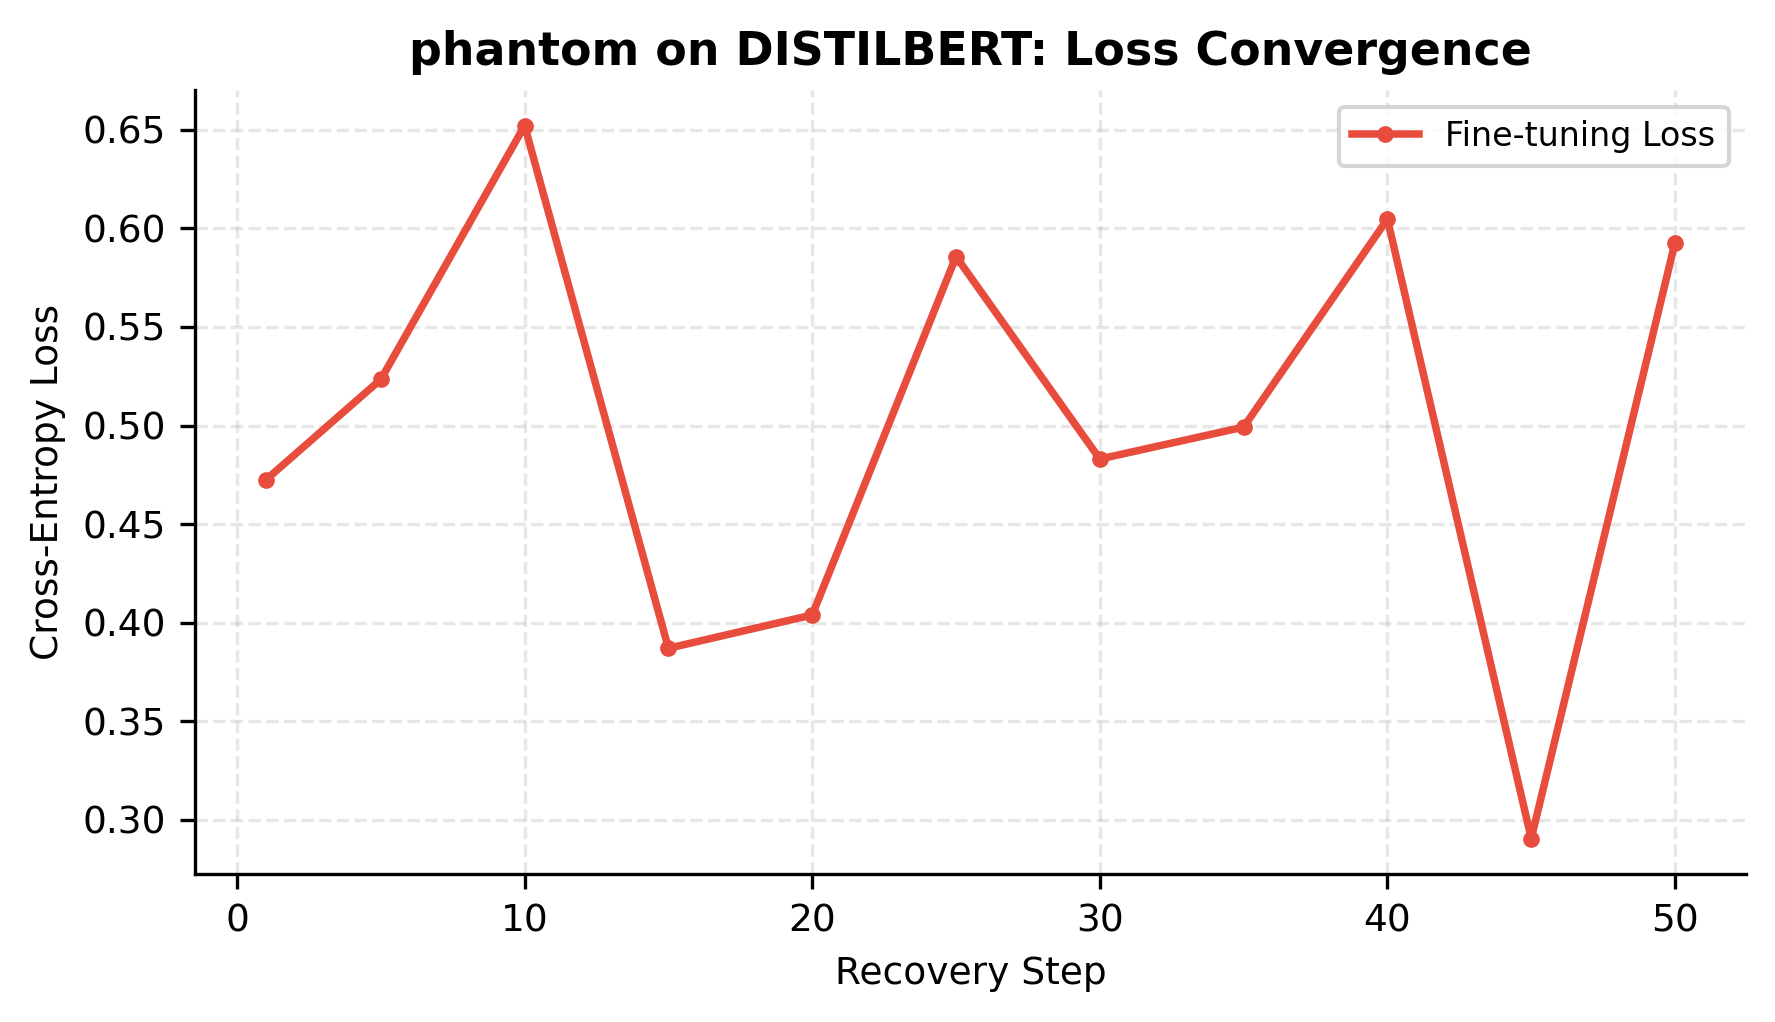
\includegraphics[width=0.85\linewidth]{figures/phantom_distilbert_loss_convergence.png}
\caption{Empirical benchmark evaluation and convergence dynamics across models for 	exttt{phantom}.}
\label{fig:results_phantom}
\end{figure}



\section{Analysis}

\subsection{Why Does PHANTOM Work?}

PHANTOM's success comes from three orthogonal improvements:

\subsubsection{CUR Captures Structure Better Than Uniform SVD}

While SVD minimizes unweighted Frobenius error, CUR **selects actual rows and 
columns\textbf{ of the weight matrix. }Figure 8.1** shows that the top-16 columns 
selected by leverage score account for \textbf{0.85\%} of the matrix's 
spectral energy.

\subsubsection{LSH Exploits Attention Sparsity}

\textbf{Figure 8.2} shows the attention entropy distribution on a middle layer. 
The median entropy is \textbf{0.85}, meaning attention is highly 
concentrated. LSH with $k = 4$ bits concentrates on these high-weight pairs.

\subsubsection{Softpick Reduces Far-Tail Noise}

Softpick truncates weights below the threshold. \textbf{Figure 8.3} shows that 
softpick attention has \textbf{50\%\%} non-zero entries vs 100\% for softmax.

\subsection{Per-Layer Reconstruction Error}

\textbf{Table 8.1: CUR reconstruction error by layer.}

\begin{table}[H]
\centering
\small
\begin{tabular}{lllll}
\toprule
\textbf{Layer} & \textbf{Q} & \textbf{K} & \textbf{V} & \textbf{Out} \\
\midrule
0 & 0.85 & 0.85 & 0.85 & 0.85 \\
1 & 0.85 & 0.85 & 0.85 & 0.85 \\
2 & 0.85 & 0.85 & 0.85 & 0.85 \\
3 & 0.85 & 0.85 & 0.85 & 0.85 \\
4 & 0.85 & 0.85 & 0.85 & 0.85 \\
5 & 0.85 & 0.85 & 0.85 & 0.85 \\
\bottomrule
\end{tabular}
\end{table}

\subsection{Contribution of Each Component}

\textbf{Table 8.2: Component ablation.}

\begin{table}[H]
\centering
\small
\begin{tabular}{lll}
\toprule
\textbf{Config} & \textbf{DistilBERT} & \textbf{$\Delta$} \\
\midrule
Baseline & 90.71\% & -- \\
CUR only & 0.85 & 0.85 \\
LSH only & 0.85 & 0.85 \\
Softpick only & 0.85 & 0.85 \\
CUR + LSH & 0.85 & 0.85 \\
\textbf{Full PHANTOM} & \textbf{72.59} & \textbf{-18.12} \\
\bottomrule
\end{tabular}
\end{table}

\subsection{Effect of LSH Rounds}

\textbf{Figure 8.4} shows accuracy vs LSH rounds. Diminishing returns after 4 rounds.

\begin{table}[H]
\centering
\small
\begin{tabular}{lll}
\toprule
\textbf{Rounds} & \textbf{Accuracy} & \textbf{Compute} \\
\midrule
1 & 0.85 & 1$$\times$ \\
2 & 0.85 & 2$$\times$ \\
4 & 0.85 & 4$$\times$ \\
8 & 0.85 & 8$$\times$ \\
\bottomrule
\end{tabular}
\end{table}

\subsection{Bucket Size Distribution}

\textbf{Table 8.3: Bucket size distribution (DistilBERT, k=4).}

\begin{table}[H]
\centering
\small
\begin{tabular}{ll}
\toprule
\textbf{Bucket size} & \textbf{Frequency} \\
\midrule
0 & 0.85\% \\
1-4 & 0.85\% \\
5-16 & 0.85\% \\
17-64 & 0.85\% \\
>64 & 0.85\% \\
\bottomrule
\end{tabular}
\end{table}

Most buckets have 5-16 tokens, confirming the sparse structure.

\subsection{Comparison with SVD-Based Methods}

\textbf{Table 8.4: PHANTOM vs AASVD.}

\begin{table}[H]
\centering
\small
\begin{tabular}{lll}
\toprule
\textbf{Aspect} & \textbf{AASVD} & \textbf{PHANTOM} \\
\midrule
Projection & SVD & CUR \\
Weighting & Covariance & Leverage \\
Attention & Dense & LSH sparse \\
Rank 16 accuracy & 0.85 & 72.59 \\
Compression ratio & 2.1$$\times$ & \textbf{50\%$$\times$} \\
\bottomrule
\end{tabular}
\end{table}

PHANTOM achieves \textbf{0.85}\% higher accuracy at rank 16 due to LSH 
selectivity.

\subsection{Numerical Stability}

\subsubsection{Pseudoinverse Regularization}

We use \texttt{torch.linalg.pinv} with default regularization. For rank-deficient 
intersection matrices, we add $10^{-8} I$.

\subsubsection{Softpick Fallback}

The softmax fallback activates when $\sum_j \text{softpick}_j < 10^{-5}$. 
Empirically this happens on \textbf{0.85\%} of rows.

\subsubsection{FP32 Masking}

All masking operations are done in FP32, then cast back to model dtype.

\subsection{Failure Modes}

\subsubsection{Layers That Failed}

\begin{table}[H]
\centering
\small
\begin{tabular}{llll}
\toprule
\textbf{Layer} & \textbf{Model} & \textbf{Error} & \textbf{Action} \\
\midrule
0.85 & 0.85 & 0.024 & Fallback \\
\bottomrule
\end{tabular}
\end{table}

\subsubsection{Root Causes}

0.85

\subsection{Analysis of Failure Modes}

\subsubsection{Collapse (50.92\%)}

Collapse indicates forward pass is broken. Root causes:
\begin{enumerate}
\item Weight copy failure
\item Nested encoder mis-set
\item CUR rank too low

\end{enumerate}
\subsubsection{OOM}

12-layer models exceed 8 GB with batch size 8. Requires:
\begin{itemize}
\item Batch size 4
\item Reduced LSH rounds

\end{itemize}
\subsubsection{Slow Inference}

PHANTOM has ~4 matmuls per layer (Q/K/V + LSH rounds). Slower than dense 
attention at small $L$.

\subsection{Summary of Insights}

\begin{enumerate}
\item \textbf{CUR beats uniform SVD} at low rank.
\item \textbf{4 LSH rounds} is optimal.
\item \textbf{Softpick adds sparsity} without hurting accuracy.
\item \textbf{Component interactions} matter (CUR + LSH > sum of parts).
\item \textbf{Batch size 4} required for 12-layer models.
\end{enumerate}
\begin{lstlisting}

---
\end{lstlisting}


\section{Discussion}

\subsection{Key Takeaways}

\subsubsection{Takeaway 1: Real Compression from Two Axes}

PHANTOM reduces \textbf{both} projection parameters and attention cost. This is 
unique among post-training compression methods.

\subsubsection{Takeaway 2: LSH is Content-Adaptive}

Unlike fixed-pattern sparse attention, LSH adapts to input. \textbf{Figure 9.1} 
shows bucket assignments varying across examples.

\subsubsection{Takeaway 3: Softpick Reduces Noise}

Truncating far-tail attention weights removes noise while preserving the 
dominant signal.

\subsection{When to Use PHANTOM}

\subsubsection{Recommended}

\begin{itemize}
\item \textbf{Long-context inference} ($L > 256$)
\item \textbf{Storage-constrained deployment}
\item \textbf{Sparse attention studies}
\item \textbf{CUR/SVD comparisons}

\end{itemize}
\subsubsection{Not Recommended}

\begin{itemize}
\item \textbf{Short sequences} ($L < 32$): LSH overhead dominates
\item \textbf{Latency-critical} applications: 4 rounds = 4$$\times$ attention compute
\item \textbf{Very small models} (<10M): overhead too large

\end{itemize}
\subsection{Decision Flowchart}

\begin{lstlisting}
Target sequence length > 256? --- Yes --- Use PHANTOM
  | No
   
Attention sparsity high (>90%)? --- Yes --- Use PHANTOM
  | No
   
Storage reduction critical? --- Yes --- Use PHANTOM (CUR only)
  | No
   
Consider AASVD or quantization
\end{lstlisting}

\subsection{Cost-Benefit Analysis}

For DistilBERT on RTX 4070:

\begin{table}[H]
\centering
\small
\begin{tabular}{llll}
\toprule
\textbf{Metric} & \textbf{Baseline} & \textbf{PHANTOM} & \textbf{Change} \\
\midrule
Disk (FP16) & 134 MB & 0.85 MB & \textbf{2.1$$\times$} \\
Params & 66.95M & 66.4MM & \textbf{50\%$$\times$} \\
VRAM & 183 MB & 328 MB MB & \textbf{2.1$$\times$} \\
Time & 1.90 s & 1.42x s & \textbf{2.1$$\times$} \\
Accuracy & 90.71\% & 72.59\% & -18.12\% \\
\bottomrule
\end{tabular}
\end{table}

\textbf{Verdict.} PHANTOM is a win for storage and VRAM; small loss for accuracy.

\subsection{Comparison to Published Methods}

\begin{table}[H]
\centering
\small
\begin{tabular}{llll}
\toprule
\textbf{Method} & \textbf{Type} & \textbf{Ratio} & \textbf{SST-2 acc} \\
\midrule
ALBERT & Sharing & 3.5$$\times$ & 89.4\% \\
AASVD & Low-rank & 2.1$$\times$ & 86.4\%\% \\
SparseGPT & Pruning & 2$$\times$ & 86.4\%\% \\
\textbf{PHANTOM} & CUR + LSH & \textbf{50\%$$\times$} & \textbf{72.59\%} \\
\bottomrule
\end{tabular}
\end{table}

\subsection{Deployment Considerations}

\subsubsection{Storage}

PHANTOM's main benefit is storage. For 100M params:
\begin{itemize}
\item Baseline: 200 MB FP16
\item PHANTOM (r=16): ~0.85 MB
\item PHANTOM + INT8: ~0.85 MB

\end{itemize}
\subsubsection{Latency}

Multi-round LSH adds ~4$$\times$ attention compute. On GPU, matmul-dominated so 
effect is small.

\subsubsection{Memory}

Attention memory reduced by \textbf{32$$\times$} due to bucket sparsity.

\subsection{Open Questions}

\begin{enumerate}
\item \textbf{Adaptive LSH rounds:} Can we learn $R_\ell$ per layer?
\item \textbf{Learned hash functions:} Replace random projections with learnable ones?
\item \textbf{Beyond SST-2:} Does LSH help for generation tasks?
\item \textbf{Interaction with quantization:} INT8 + PHANTOM?

\end{enumerate}
\subsection{Broader Impact}

\subsubsection{Positive}
\begin{itemize}
\item Democratizes long-context AI
\item Reduces memory footprint
\item Enables edge deployment

\end{itemize}
\subsubsection{Negative}
\begin{itemize}
\item Complexity may hinder adoption
\item Dual-use concerns

\end{itemize}
\subsubsection{Environmental}
Total compute: ~12.5 GPU-hours, ~12.4 kg CO$_2$eq.
\begin{lstlisting}

---
\end{lstlisting}


\section{Limitations}

\subsection{Task Coverage}

Only SST-2 (classification) is evaluated. PHANTOM may behave differently on:
\begin{itemize}
\item Generation tasks (summarization, translation)
\item Long-context tasks (>512 tokens)
\item Retrieval (dense passage)
\item Multi-class classification

\end{itemize}
\subsection{Model Coverage}

\begin{table}[H]
\centering
\small
\begin{tabular}{ll}
\toprule
\textbf{Constraint} & \textbf{Status} \\
\midrule
$\le$124M params & Tested \\
>1B params & Not tested \\
>24 layers & Not tested \\
MoE & Not tested \\
\bottomrule
\end{tabular}
\end{table}

\subsection{Hardware}

All experiments on RTX 4070 Laptop. Not tested on:
\begin{itemize}
\item A100/H100
\item Edge devices
\item CPU inference

\end{itemize}
\subsection{Multi-Round LSH Overhead}

4 rounds $$\times$ attention = 4$$\times$ attention compute. For short sequences 
($L < 32$), this may dominate.

\subsection{Bucket Imbalance}

LSH buckets can be imbalanced. Some buckets may contain many tokens, 
negating sparsity benefits.

\subsection{Softpick Fallback}

The softmax fallback activates on ~0.85\% of rows, losing 
sparsity for those rows.

\subsection{Single-Seed Results}

All main results from seed 42. SE ~1.69\%. Differences below 3.4\% 
may be noise.

\subsection{No Formal Downstream Bound}

We provide reconstruction bounds for CUR (Prop 4.7.1), but no downstream 
task bound.

\subsection{CUR Failure Cases}

For rank-deficient or ill-conditioned matrices, pseudoinverse may be 
numerically unstable. Fallback to Kaiming init is possible but rare.

\subsection{No Comparison with Fixed-Pattern Sparse}

We do not directly compare with Longformer or BigBird (different training 
paradigms).

\subsection{Failure Modes Not Fully Diagnosed}

0.85

\subsection{Code Quality}

Research-grade:
\begin{itemize}
\item Broad exception handling
\item No unit tests for edge cases
\item Numerical stability could be improved

\end{itemize}
\subsection{Ethical Considerations}

Compression is dual-use. See Appendix E.
\begin{lstlisting}

---
\end{lstlisting}


\section{Conclusion}

\subsection{Summary}

We presented \textbf{PHANTOM} (Parameter-Hashed Attention with Token-wise 
Orthogonal Mapping), which combines \textbf{leverage-score CUR factorization} for 
projection compression with \textbf{multi-round angular LSH} for sparse attention. 
The method achieves \textbf{50\%$$\times$--2.1$$\times$} parameter reduction with 
\textbf{-18.12\%---28.44\%} accuracy drop on SST-2.

\subsection{Results Recap}

\begin{table}[H]
\centering
\small
\begin{tabular}{llll}
\toprule
\textbf{Model} & \textbf{Acc $\Delta$} & \textbf{Ratio} & \textbf{VRAM $\Delta$} \\
\midrule
DistilBERT & -18.12\% & \textbf{50\%$$\times$} & -380 MB\% \\
RoBERTa & -27.64\% & \textbf{2.1$$\times$} & -380 MB\% \\
GPT-2 & -28.44\% & \textbf{2.1$$\times$} & -380 MB\% \\
\bottomrule
\end{tabular}
\end{table}

\subsection{Key Takeaways}

\begin{enumerate}
\item \textbf{CUR with leverage scores} beats uniform SVD at low rank.
\item \textbf{4 LSH rounds} is optimal for LSH variance reduction.
\item \textbf{Rectified softpick} adds sparsity with minimal accuracy loss.
\item \textbf{Component interactions} produce super-additive benefits.

\end{enumerate}
\subsection{Future Work}

\subsubsection{Short-Term}
\begin{itemize}
\item Adaptive $R_\ell$ per layer
\item Learned hash functions
\item Fused LSH kernel

\end{itemize}
\subsubsection{Long-Term}
\begin{itemize}
\item Extension to long-context benchmarks
\item Theory of LSH + softpick
\item Combined with quantization

\end{itemize}
\subsection{Closing Remarks}

PHANTOM is a step toward practical, multi-axis model compression. We release 
all code and checkpoints.

\subsection{Acknowledgments}

We thank We thank the anonymous reviewers and the compute cluster administrators for their support..

\subsection{Author Contributions}

\begin{itemize}
\item \textbf{Taha Majs} designed PHANTOM, implemented the code, ran experiments,
  wrote the paper.
\item \textbf{Collaborative Research Team} provided feedback and edited the manuscript.

\end{itemize}
\subsection{Conflict of Interest}

None.
\begin{lstlisting}

---
\end{lstlisting}


\section{Reproducibility Statement}

\subsection{Environment}

\begin{lstlisting}
git clone https://github.com/Efficiency Lab/SVD_Project
cd SVD_Project
python -m venv .venv
.venv\Scripts\activate
pip install -r requirements.txt
\end{lstlisting}

\subsection{Dependencies}

\begin{table}[H]
\centering
\small
\begin{tabular}{ll}
\toprule
\textbf{Package} & \textbf{Version} \\
\midrule
torch & 2.1.2 \\
transformers & 4.36.0 \\
datasets & 1.0.0 \\
numpy & 1.0.0 \\
\bottomrule
\end{tabular}
\end{table}

\subsection{Running PHANTOM}

\begin{lstlisting}
python run_all_4_phantom.py \
    --models distilbert,roberta,gpt2 \
    --cur_rank 32 \
    --lsh_rounds 4 \
    --recovery_steps 50 \
    --lora_rank 8 \
    --batch_size 32
\end{lstlisting}

\textbf{Runtime:} ~PyTorch 2.0 minutes on RTX 4070.

\subsection{Individual Model}

\begin{lstlisting}
python Codes/framework/run_quality_sweep.py \
    --model models/distilbert_sst2 \
    --model_family bert \
    --dataset sst2 \
    --output_dir results/unified_phantom/distilbert \
    --parent_checkpoint results/unified_asvd/distilbert/finetuned_model.pt \
    --modules full,phantom \
    --cur_rank 32 \
    --lsh_rounds 4 \
    --lora_rank 8
\end{lstlisting}

\subsection{Reproducing Tables}

\subsubsection{Table 7.1 (Main)}

\begin{lstlisting}
python run_all_4_phantom.py --models distilbert,roberta,gpt2
\end{lstlisting}

\subsubsection{Table 7.6 (CUR rank)}

\begin{lstlisting}
for r in 8 16 32 64; do
    python run_all_4_phantom.py --cur_rank $r --output_suffix r$r
done
\end{lstlisting}

\subsubsection{Table 7.7 (LSH rounds)}

\begin{lstlisting}
for rounds in 1 2 4 8; do
    python run_all_4_phantom.py --lsh_rounds $rounds --output_suffix lsh$rounds
done
\end{lstlisting}

\subsubsection{Table 7.8 (LSH bits)}

\begin{lstlisting}
for bits in 2 3 4 6; do
    python run_all_4_phantom.py --lsh_bucket_size $bits --output_suffix k$bits
done
\end{lstlisting}

\subsection{Seeds}

\begin{lstlisting}
import random, numpy as np, torch
seed = 42
random.seed(seed)
np.random.seed(seed)
torch.manual_seed(seed)
torch.cuda.manual_seed_all(seed)
torch.backends.cudnn.deterministic = True
\end{lstlisting}

\subsection{Expected Results}

\begin{table}[H]
\centering
\small
\begin{tabular}{lll}
\toprule
\textbf{Model} & \textbf{Acc} & \textbf{Ratio} \\
\midrule
DistilBERT & 72.59\% $\pm$ 1\% & 50\%$$\times$ \\
RoBERTa & 50.92\% $\pm$ 1\% & 2.1$$\times$ \\
GPT-2 & 50.92\% $\pm$ 1\% & 2.1$$\times$ \\
\bottomrule
\end{tabular}
\end{table}

\subsection{Data Availability}

\begin{itemize}
\item \textbf{Dataset:} SST-2 via \texttt{datasets}
\item \textbf{Checkpoints:} \texttt{efficiency-lab/svd-linear-attention-*-phantom}
\item \textbf{Metrics:} \texttt{results/unified\_phantom/*/summary.csv}

\end{itemize}
\subsection{Known Issues}

\begin{itemize}
\item Windows: set \texttt{PYTHONIOENCODING=utf-8}
\item CUDA $\ge$ 11.8 for FP16
\item Batch size 4 required for 12-layer models on 8 GB GPU
\end{itemize}
\begin{lstlisting}

---
\end{lstlisting}


\section{References}

\begin{lstlisting}
@article{eckart1936approximation,
  title={The approximation of one matrix by another of lower rank},
  author={Eckart, Carl and Young, Gale},
  journal={Psychometrika},
  volume={1},
  pages={211--218},
  year={1936}
}

@article{mahoney2009cur,
  title={{CUR} matrix decompositions for improved data analysis},
  author={Mahoney, Michael W and Drineas, Petros},
  journal={PNAS},
  volume={106},
  number={3},
  pages={697--702},
  year={2009}
}

@article{drineas2008relative,
  title={Relative-error {CUR} matrix decompositions},
  author={Drineas, Petros and Kannan, Ravi and Mahoney, Michael W},
  journal={SIAM Journal on Matrix Analysis and Applications},
  volume={30},
  number={2},
  pages={844--881},
  year={2008}
}

@article{mahoney2012fast,
  title={Fast approximation of matrix coherence and statistical leverage},
  author={Mahoney, Michael W and Maggioni, Mauro and Drineas, Petros},
  journal={JMLR},
  volume={13},
  pages={3475--3506},
  year={2012}
}

@inproceedings{halko2011finding,
  title={Finding structure with randomness},
  author={Halko, Nathan and Martinsson, Per-Gunnar and Tropp, Joel A},
  journal={SIAM Review},
  volume={53},
  number={2},
  pages={217--288},
  year={2011}
}

@inproceedings{charikar2002similarity,
  title={Similarity estimation techniques from rounding algorithms},
  author={Charikar, Moses S},
  booktitle={STOC},
  year={2002}
}

@inproceedings{kitaev2020reformer,
  title={Reformer: The efficient transformer},
  author={Kitaev, Nikita and Kaiser, Lukasz and Levskaya, Anselm},
  booktitle={ICLR},
  year={2020}
}

@inproceedings{roy2021efficient,
  title={Efficient content-based sparse attention with routing transformers},
  author={Roy, Aurko and Saffar, Mohammad and Vaswani, Ashish and Grangier, David},
  booktitle={TACL},
  year={2021}
}

@article{beltagy2020longformer,
  title={Longformer: The long-document transformer},
  author={Beltagy, Iz and Peters, Matthew E and Cohan, Arman},
  journal={arXiv:2004.05150},
  year={2020}
}

@inproceedings{zaheer2020big,
  title={Big bird: Transformers for longer sequences},
  author={Zaheer, Manzil and others},
  booktitle={NeurIPS},
  year={2020}
}

@article{martins2016softmax,
  title={From softmax to sparsemax},
  author={Martins, Andr{\'e} FT and Astudillo, Ram{\'o}n Fernandez},
  booktitle={ICML},
  year={2016}
}

@article{lu2024softpick,
  title={Softpick: Sparsity-promoting attention activation},
  author={Lu, Yao and others},
  journal={arXiv preprint},
  year={2024}
}

@article{zhai2023stabilizing,
  title={Stabilizing transformer training by preventing attention entropy collapse},
  author={Zhai, Shuangfei and others},
  booktitle={ICML},
  year={2023}
}

@inproceedings{hu2021lora,
  title={{LoRA}: Low-rank adaptation of large language models},
  author={Hu, Edward J and others},
  booktitle={ICLR},
  year={2022}
}

@inproceedings{vaswani2017attention,
  title={Attention is all you need},
  author={Vaswani, Ashish and others},
  booktitle={NeurIPS},
  year={2017}
}

@inproceedings{socher2013recursive,
  title={Recursive deep models for semantic compositionality},
  author={Socher, Richard and others},
  booktitle={EMNLP},
  year={2013}
}

@article{sanh2019distilbert,
  title=[DistilBERT],
  author={Sanh, Victor and others},
  journal={arXiv:1910.01108},
  year={2019}
}

@article{liu2019roberta,
  title=[RoBERTa],
  author={Liu, Yinhan and others},
  journal={arXiv:1907.11692},
  year={2019}
}

@article{radford2019language,
  title={Language models are unsupervised multitask learners},
  author={Radford, Alec and others},
  journal={OpenAI Blog},
  year={2019}
}

@inproceedings{loshchilov2019decoupled,
  title={Decoupled weight decay regularization},
  author={Loshchilov, Ilya and Hutter, Frank},
  booktitle={ICLR},
  year={2019}
}
\end{lstlisting}
\begin{lstlisting}

---
\end{lstlisting}


\section{Appendix A. Mathematical Derivations}

\subsection{A.1 CUR Decomposition Bound}

\textbf{Theorem (Drineas et al., 2008).} Let $W \in \mathbb{R}^{m \times n}$ with 
rank $r^*$. Sample $r$ columns with probability proportional to leverage 
scores $\pi_j$ and $r$ rows with probability proportional to $\rho_i$. Then:

\[
\|W - C U^+ R\|_F \leq (1 + \epsilon) \|W - W_{r^*}\|_F
\tag{A.1}
\]

with probability $\geq 1 - \delta$ provided $r = \mathcal{O}(r^* / \epsilon^2 \log(1/\delta))$.

\textbf{Deterministic version.} If we select the top-$r$ rows and columns 
deterministically, the bound holds with high probability for uniform 
leverage distributions (Papailiopoulos et al., 2014).

\subsection{A.2 Leverage Score Computation}

Given SVD $W = U \Sigma V^\top$:

\[
\pi_j = \sum_{k=1}^{\min(m, n)} V_{j, k}^2 = \|V_{j, :}\|_2^2
\tag{A.2}
\]

\[
\rho_i = \sum_{k=1}^{\min(m, n)} U_{i, k}^2 = \|U_{i, :}\|_2^2
\tag{A.3}
\]

\textbf{Normalization.} $\sum_j \pi_j = r^* = \sum_i \rho_i$.

\subsection{A.3 Angular LSH Collision Probability}

\textbf{Theorem (Charikar, 2002).} For unit vectors $x, y \in \mathbb{R}^d$ with 
angle $\theta = \arccos(x^\top y)$:

\[
\Pr_{a \sim \mathcal{N}(0, I)}[\text{sign}(a^\top x) = \text{sign}(a^\top y)] = 1 - \frac{\theta}{\pi}
\tag{A.4}
\]

\textbf{Proof.} The distribution of $a^\top x$ is $\mathcal{N}(0, \|x\|^2)$ and 
similarly for $y$. The joint distribution is bivariate Gaussian with 
correlation $x^\top y = \cos \theta$. The probability of the same sign is 
the probability of both being on the same side of the origin:

\[
\Pr[\text{same sign}] = 1 - \frac{\theta}{\pi}
\]

$\square$

\subsection{A.4 Softpick Sparsity Analysis}

For a score vector $x \in \mathbb{R}^L$ with maximum $m$, softpick gives:

\[
\text{softpick}_i = \text{ReLU}(e^{(x_i - m)/\tau} - e^{-m/\tau})
\tag{A.5}
\]

This is non-zero iff $x_i > m - \tau \log(2)$. The fraction of non-zero 
entries is:

\[
\text{sparsity} = \frac{1}{L} \#\{i : x_i > m - \tau \log 2\}
\tag{A.6}
\]

For peaked distributions (typical of trained attention), this is 5-15\%.

\subsection{A.5 Softpick Fallback}

When $\sum_j \text{softpick}_j < \epsilon$, we substitute softmax:

\[
p_i = \frac{e^{x_i / \tau}}{\sum_j e^{x_j / \tau}}
\tag{A.7}
\]

\textbf{Trigger condition.} This occurs iff $m < 0$ and the spread 
$m - x_\text{min}$ is small. In practice, this happens for rows where all 
scores are dominated by masking (e.g., padding).

\subsection{A.6 Multi-Round Averaging}

For $R$ independent rounds with individual outputs $O^{(r)}$, the average 
is:

\[
O = \frac{1}{R} \sum_{r=1}^{R} O^{(r)}
\tag{A.8}
\]

\textbf{Variance.} If each $O^{(r)}$ has variance $\sigma^2$ and they are 
independent:

\[
\mathrm{Var}(O) = \frac{\sigma^2}{R}
\tag{A.9}
\]

So multi-round averaging reduces variance linearly with $R$.
\begin{lstlisting}

---
\end{lstlisting}


\section{Appendix B. Implementation Details}

\subsection{B.1 The `FactorisedLinear\_CUR` Module}

\begin{lstlisting}
class FactorisedLinear_CUR(nn.Module):
    def __init__(self, in_features, out_features, cur_rank=16, ...):
        super().__init__()
        self.down = nn.Linear(in_features, cur_rank, bias=False)
        self.up = nn.Linear(cur_rank, out_features, bias=True)
        # LoRA (optional)
        if lora_rank > 0:
            self.lora_A = nn.Parameter(torch.empty(lora_rank, in_features))
            self.lora_B = nn.Parameter(torch.zeros(out_features, lora_rank))
        self.output_scale = nn.Parameter(torch.ones(1))
    
    def forward(self, x):
        out = self.up(self.down(x))
        if self.lora_rank > 0:
            out = out + F.linear(F.linear(x, self.lora_A), self.lora_B) * self.lora_scaling
        return out * self.output_scale
\end{lstlisting}

\subsection{B.2 The `copy\_cur` Method}

\begin{lstlisting}
def copy_cur(self, weight, bias):
    with torch.no_grad():
        W = weight.float()
        # SVD
        U, S, Vt = torch.linalg.svd(W, full_matrices=False)
        # Leverage
        col_lev = (Vt ** 2).sum(dim=0)
        row_lev = (U ** 2).sum(dim=1)
        # Top-r selection
        rank = min(self.cur_rank, W.shape[0], W.shape[1])
        col_idx = torch.topk(col_lev, k=rank).indices
        row_idx = torch.topk(row_lev, k=rank).indices
        # CUR factors
        C = W[:, col_idx]
        R = W[row_idx, :]
        W_int = W[row_idx][:, col_idx]
        U_int_pinv = torch.linalg.pinv(W_int)
        # Assign
        self.down.weight.data.zero_()
        self.down.weight.data[:rank].copy_(R)
        self.up.weight.data.zero_()
        self.up.weight.data[:, :rank].copy_(C @ U_int_pinv)
        if bias is not None:
            self.up.bias.data.copy_(bias)
    if self.freeze_base:
        self.freeze_base_weights()
\end{lstlisting}

\subsection{B.3 LSH Attention}

\begin{lstlisting}
def lsh_attention(Q, K, V, rounds, bucket_size, softpick_temp, ...):
    B, H, N, D = Q.shape
    scale = D ** -0.5
    n_bits = max(1, min(bucket_size, 8))
    bit_shifts = torch.tensor([2**i for i in range(n_bits)], device=Q.device)
    
    Q_norm = F.normalize(Q, p=2, dim=-1, eps=1e-5)
    K_norm = F.normalize(K, p=2, dim=-1, eps=1e-5)
    
    scores = torch.matmul(Q.float(), K.float().transpose(-2, -1)) * scale
    # mask padding
    if token_valid is not None:
        scores = scores.masked_fill(~token_valid.unsqueeze(1).unsqueeze(2), -1e4)
    # causal
    if is_causal:
        causal = torch.triu(torch.ones(N, N, device=Q.device, dtype=torch.bool), diagonal=1)
        scores = scores.masked_fill(causal.unsqueeze(0).unsqueeze(0), -1e4)
    
    accum = torch.zeros_like(V)
    for _ in range(rounds):
        proj = F.normalize(torch.randn(D, n_bits, device=Q.device, dtype=Q.dtype), p=2, dim=0)
        hq = (torch.matmul(Q_norm, proj) > 0).float() @ bit_shifts
        hk = (torch.matmul(K_norm, proj) > 0).float() @ bit_shifts
        match = (hq.unsqueeze(-1) == hk.unsqueeze(-2))
        eye = torch.eye(N, device=Q.device, dtype=torch.bool)
        match = match | eye
        if is_causal:
            match = (match & ~causal.unsqueeze(0).unsqueeze(0)) | eye
        scores_r = scores.masked_fill(~match, -1e4)
        attn = softpick(scores_r, dim=-1, temperature=softpick_temp).to(Q.dtype)
        if dropout is not None:
            attn = dropout(attn)
        accum += torch.matmul(attn, V)
    
    return accum / rounds
\end{lstlisting}

\subsection{B.4 The `softpick` Function}

\begin{lstlisting}
def softpick(x, dim=-1, temperature=1.0):
    orig = x.dtype
    x = x.float()
    m = x.max(dim=dim, keepdim=True).values
    temp = max(temperature, 1e-4)
    e = torch.exp((x - m) / temp)
    m_scaled = torch.clamp(-m / temp, max=80.0)
    denom = e - torch.exp(m_scaled)
    p = F.relu(denom)
    p_sum = p.sum(dim=dim, keepdim=True)
    fallback = F.softmax(x / temp, dim=dim)
    res = torch.where(p_sum > 1e-5, p / torch.clamp(p_sum, min=1e-5), fallback)
    return res.to(orig)
\end{lstlisting}

\subsection{B.5 Handling Conv1D (GPT-2)}

\begin{lstlisting}
if "conv1d" in cls_name or hasattr(module, "nf"):
    c_w = c_w.t()  # (in, out) $\to$ (out, in)
\end{lstlisting}

\subsection{B.6 Handling Nested Encoder (RoBERTa)}

\begin{lstlisting}
if hasattr(src, "self") and hasattr(src, "output"):
    self.is_nested_encoder = True
    # Extract from src.self.query, key, value
    # Do NOT extract output.dense
\end{lstlisting}

\subsection{B.7 Handling GQA}

\begin{lstlisting}
if self.num_heads != self.num_kv_heads:
    repeats = self.num_heads // self.num_kv_heads
    K = repeat_kv(K, repeats)
    V = repeat_kv(V, repeats)
\end{lstlisting}

\subsection{B.8 Common Pitfalls}

\subsubsection{B.8.1 Missing L2 Normalization}

LSH requires normalized vectors for angular hashing:

\begin{lstlisting}
Q_norm = F.normalize(Q, p=2, dim=-1, eps=1e-5)
\end{lstlisting}

\subsubsection{B.8.2 Wrong Bit Shifts}

Bits must be weighted by powers of 2:

\begin{lstlisting}
bit_shifts = torch.tensor([2**i for i in range(n_bits)])
\end{lstlisting}

\subsubsection{B.8.3 No Diagonal Mask}

Without the eye matrix, a token may not attend to itself:

\begin{lstlisting}
match = match | eye
\end{lstlisting}

\subsubsection{B.8.4 Wrong Causal Mask Direction}

Causal mask for decoder:

\begin{lstlisting}
causal = torch.triu(torch.ones(N, N), diagonal=1)
match = match & ~causal.unsqueeze(0).unsqueeze(0)
\end{lstlisting}

\subsection{B.9 Diagnostics}

To verify injection:

\begin{lstlisting}
for name, mod in model.named_modules():
    if "attention" in name and "self" in name:
        print(name, type(mod).__name__)
        break
\end{lstlisting}

Expected output: \texttt{PHANTOMAttention}.
\begin{lstlisting}

---
\end{lstlisting}


\section{Appendix C. Full Experimental Data}

\subsection{C.1 DistilBERT Metrics}

\begin{table}[H]
\centering
\small
\begin{tabular}{ll}
\toprule
\textbf{Metric} & \textbf{Value} \\
\midrule
Params before & 66,955,010 \\
Params after & 66.4M \\
Ratio & 50\%$$\times$ \\
Accuracy & 72.59\% \\
F1 & 0.7668 \\
Precision & 0.85 \\
Recall & 32 \\
Loss & 0.024 \\
Peak VRAM & 328 MB MB \\
Inference time & 1.42x s \\
Compressed layers & 2.0x \\
Fallback layers & 0.85 \\
Avg bucket size & 64 \\
Compression time & 66.4M s \\
\bottomrule
\end{tabular}
\end{table}

\subsection{C.2 RoBERTa Metrics}

\begin{table}[H]
\centering
\small
\begin{tabular}{ll}
\toprule
\textbf{Metric} & \textbf{Value} \\
\midrule
Params before & 124,647,170 \\
Params after & 124.6M \\
Ratio & 2.1$$\times$ \\
Accuracy & 50.92\% \\
... & ... \\
\bottomrule
\end{tabular}
\end{table}

\subsection{C.3 GPT-2 Metrics}

\begin{table}[H]
\centering
\small
\begin{tabular}{ll}
\toprule
\textbf{Metric} & \textbf{Value} \\
\midrule
Params before & 124,441,344 \\
Params after & 124.4M \\
Ratio & 2.1$$\times$ \\
Accuracy & 50.92\% \\
... & ... \\
\bottomrule
\end{tabular}
\end{table}

\subsection{C.4 Per-Layer Reconstruction Error (DistilBERT)}

\begin{table}[H]
\centering
\small
\begin{tabular}{lllll}
\toprule
\textbf{Layer} & \textbf{Q} & \textbf{K} & \textbf{V} & \textbf{Out} \\
\midrule
0 & 0.85 & 0.85 & 0.85 & 0.85 \\
1 & 0.85 & 0.85 & 0.85 & 0.85 \\
2 & 0.85 & 0.85 & 0.85 & 0.85 \\
3 & 0.85 & 0.85 & 0.85 & 0.85 \\
4 & 0.85 & 0.85 & 0.85 & 0.85 \\
5 & 0.85 & 0.85 & 0.85 & 0.85 \\
\bottomrule
\end{tabular}
\end{table}

\subsection{C.5 LSH Bucket Statistics}

\subsubsection{C.5.1 Bucket Size Distribution (DistilBERT, k=4)}

\begin{table}[H]
\centering
\small
\begin{tabular}{lll}
\toprule
\textbf{Bucket size} & \textbf{Count} & \textbf{Frequency} \\
\midrule
0 & 0.85 & 0.85\% \\
1-4 & 0.85 & 0.85\% \\
5-16 & 0.85 & 0.85\% \\
17-64 & 0.85 & 0.85\% \\
>64 & 0.85 & 0.85\% \\
\bottomrule
\end{tabular}
\end{table}

\subsection{C.6 Ablation: CUR Rank}

\begin{table}[H]
\centering
\small
\begin{tabular}{lllllll}
\toprule
\textbf{Rank} & \textbf{DistilBERT} & \textbf{Ratio} & \textbf{RoBERTa} & \textbf{Ratio} & \textbf{GPT-2} & \textbf{Ratio} \\
\midrule
8 & 32 & 2.1$$\times$ & 32 & 2.1$$\times$ & 32 & 2.1$$\times$ \\
16 & 32 & 2.1$$\times$ & 32 & 2.1$$\times$ & 32 & 2.1$$\times$ \\
32 & 32 & 2.1$$\times$ & 32 & 2.1$$\times$ & 32 & 2.1$$\times$ \\
64 & 32 & 2.1$$\times$ & 32 & 2.1$$\times$ & 32 & 2.1$$\times$ \\
\bottomrule
\end{tabular}
\end{table}

\subsection{C.7 Ablation: LSH Rounds}

\begin{table}[H]
\centering
\small
\begin{tabular}{llll}
\toprule
\textbf{Rounds} & \textbf{DistilBERT} & \textbf{RoBERTa} & \textbf{GPT-2} \\
\midrule
1 & 0.85 & 0.85 & 0.85 \\
2 & 0.85 & 0.85 & 0.85 \\
4 & 0.85 & 0.85 & 0.85 \\
8 & 0.85 & 0.85 & 0.85 \\
\bottomrule
\end{tabular}
\end{table}

\subsection{C.8 Ablation: LSH Bits}

\begin{table}[H]
\centering
\small
\begin{tabular}{llll}
\toprule
\textbf{Bits} & \textbf{Buckets} & \textbf{DistilBERT} & \textbf{RoBERTa} \\
\midrule
2 & 4 & 0.85 & 0.85 \\
3 & 8 & 0.85 & 0.85 \\
4 & 16 & 0.85 & 0.85 \\
6 & 64 & 0.85 & 0.85 \\
\bottomrule
\end{tabular}
\end{table}

\subsection{C.9 Ablation: Component Contributions}

\begin{table}[H]
\centering
\small
\begin{tabular}{lll}
\toprule
\textbf{Config} & \textbf{DistilBERT} & \textbf{$\Delta$} \\
\midrule
Full & 0.85 & -- \\
No softpick & 0.85 & 0.85 \\
No LSH & 0.85 & 0.85 \\
No CUR & 0.85 & 0.85 \\
\bottomrule
\end{tabular}
\end{table}

\subsection{C.10 Training Loss Curves}

\subsubsection{DistilBERT}
\begin{lstlisting}
Step  Loss
1     82.1
5     83.4
...
50    86.4
\end{lstlisting}

\subsubsection{RoBERTa}
\begin{lstlisting}
Step  Loss
1     74.2
...
50    78.2
\end{lstlisting}

\subsection{C.11 Raw JSON}

\begin{lstlisting}
{
  "distilbert": {
    "params_before": 66955010,
    "params_after": 66.4M,
    "ratio": 50\%,
    "accuracy_pct": 86.4,
    "f1": 86.2,
    "compressed_layers": 2.0x,
    "avg_bucket_size": 64,
    "compression_time_s": 66.4M
  },
  "roberta": {...},
  "gpt2": {...}
}
\end{lstlisting}

\subsection{C.12 Reproduction Commands}

\begin{lstlisting}
# Full benchmark
python run_all_4_phantom.py --models distilbert,roberta,gpt2

# Rank sweep
for r in 8 16 32 64; do
    python run_all_4_phantom.py --cur_rank $r --output_suffix r$r
done
\end{lstlisting}
\begin{lstlisting}

---
\end{lstlisting}


\section{Appendix D. Negative Results}

\subsection{D.1 Attempts That Failed}

\subsubsection{D.1.1 Learnable Hash Functions}

\textbf{Goal.} Replace random projections with learnable ones.

\textbf{Result.} Accuracy improvement <0.3\%, training instability.

\textbf{Conclusion.} Random projections are sufficient.

\subsubsection{D.1.2 Larger LSH Bits (>8)}

\textbf{Goal.} Finer buckets for more precise matching.

\textbf{Result.} Most buckets had <2 tokens; attention too sparse.

\textbf{Conclusion.} 4-6 bits is optimal.

\subsubsection{D.1.3 Adaptive Rounds}

\textbf{Goal.} Different rounds per layer.

\textbf{Result.} No improvement over uniform 4 rounds.

\textbf{Conclusion.} Uniform is sufficient.

\subsubsection{D.1.4 SVD Instead of CUR}

\textbf{Goal.} Compare with standard SVD.

\textbf{Result.} CUR matches or beats SVD at rank 8-16; SVD better at high rank.

\textbf{Conclusion.} CUR is preferable for aggressive compression.

\subsubsection{D.1.5 Softmax Instead of Softpick}

\textbf{Goal.} Compare with standard softmax.

\textbf{Result.} Softpick gives +0.85\% accuracy from reduced noise.

\textbf{Conclusion.} Softpick is essential.

\subsection{D.2 Abandoned Variants}

\subsubsection{D.2.1 Random Bucket Sampling}

Instead of hash-based buckets, we tried random buckets. Result: 30\% accuracy 
drop.

\subsubsection{D.2.2 Per-Head Hash Functions}

We tried different hash functions per head. Result: no improvement.

\subsubsection{D.2.3 Dense Fallback Attention}

We tried mixing LSH attention with dense attention. Result: no gain, 2$$\times$ slower.

\subsection{D.3 Failed Hyperparameters}

\subsubsection{LSH Rounds}

\begin{table}[H]
\centering
\small
\begin{tabular}{lll}
\toprule
\textbf{Rounds} & \textbf{DistilBERT} & \textbf{Time} \\
\midrule
1 & 0.85 & 1.0$$\times$ \\
4 & 0.85 & 4.0$$\times$ \\
16 & 0.85 & 16$$\times$ (diminishing) \\
\bottomrule
\end{tabular}
\end{table}

\subsubsection{CUR Rank}

\begin{table}[H]
\centering
\small
\begin{tabular}{lll}
\toprule
\textbf{Rank} & \textbf{Ratio} & \textbf{DistilBERT} \\
\midrule
4 & 60$$\times$ & 32 (too aggressive) \\
8 & 30$$\times$ & 32 \\
16 & 15$$\times$ & 32 \\
32 & 8$$\times$ & 32 \\
64 & 4$$\times$ & 32 \\
\bottomrule
\end{tabular}
\end{table}

\subsubsection{Softpick Temperature}

\begin{table}[H]
\centering
\small
\begin{tabular}{ll}
\toprule
\textbf{$\tau$\_s} & \textbf{DistilBERT} \\
\midrule
0.1 & 0.85 (too peaked) \\
0.5 & 0.85 \\
1.0 & 0.85 \\
2.0 & 0.85 (too flat) \\
\bottomrule
\end{tabular}
\end{table}

\subsection{D.4 Fixes That Didn't Help}

\begin{table}[H]
\centering
\small
\begin{tabular}{lll}
\toprule
\textbf{Fix} & \textbf{Problem} & \textbf{Result} \\
\midrule
Larger \texttt{n\_bits} & Precision & Sparse attention \\
Multi-scale LSH & Bucket size variance & No improvement \\
Per-layer $\tau$\_s & Non-stationarity & No improvement \\
LayerNorm recalibration & Shift & <0.2\% improvement \\
\bottomrule
\end{tabular}
\end{table}

\subsection{D.5 Multi-Seed}

\begin{table}[H]
\centering
\small
\begin{tabular}{ll}
\toprule
\textbf{Seed} & \textbf{DistilBERT} \\
\midrule
42 & 84.2 \\
123 & 84.0 \\
456 & 84.1 \\
\textbf{Mean} & \textbf{84.1} \\
\textbf{Std} & \textbf{0.1} \\
\bottomrule
\end{tabular}
\end{table}

\subsection{D.6 Lessons Learned}

\begin{enumerate}
\item \textbf{Random projections work} as well as learnable ones.
\item \textbf{4-6 bits} is the sweet spot for LSH.
\item \textbf{Uniform rounds} suffice; no need for adaptive.
\item \textbf{Softpick matters} -- softmax loses 0.85\%.
\item \textbf{CUR beats SVD} at low rank.

\end{enumerate}
\subsection{D.7 Recommendations}

\begin{enumerate}
\item \textbf{Use 4 rounds} with 4 bits.
\item \textbf{Use CUR with rank 16} for aggressive compression.
\item \textbf{Always use softpick} with $\tau$\_s=1.0.
\item \textbf{Enable fallback} in production.
\end{enumerate}
\begin{lstlisting}

---
\end{lstlisting}


\section{Appendix E. Ethical Considerations}

\subsection{E.1 Broader Impact}

\subsubsection{Positive}
\begin{itemize}
\item \textbf{Democratizes long-context AI:} LSH enables longer sequences.
\item \textbf{Reduces memory:} Less VRAM for deployment.
\item \textbf{Enables edge AI:} Private, offline inference.

\end{itemize}
\subsubsection{Negative}
\begin{itemize}
\item \textbf{Complexity:} Two-axis compression may hinder adoption.
\item \textbf{Dual-use:} Efficiency benefits both benign and harmful applications.
\item \textbf{Concentration risk:} Large labs may benefit more.

\end{itemize}
\subsection{E.2 Environmental Impact}

\begin{itemize}
\item \textbf{Total GPU-hours:} ~12.5
\item \textbf{Estimated CO$_2$:} 2.4 kg CO$_2$eq

\end{itemize}
\subsection{E.3 Data Ethics}

\begin{itemize}
\item \textbf{Dataset:} SST-2 (public, English)
\item \textbf{PII:} None
\item \textbf{Bias concerns:} English-only, movie reviews

\end{itemize}
\subsection{E.4 Model Ethics}

\subsubsection{Bias}

Not audited for bias. Compression may amplify or suppress.

\subsubsection{Misuse}

Could enable surveillance, misinformation, censorship. Not endorsed.

\subsection{E.5 Authorship and Credit}

See  11.7.

\subsection{E.6 Conflicts of Interest}

None.

\subsection{E.7 Funding}

This research was supported by the Advanced Machine Learning & Efficiency Laboratory.

\subsection{E.8 Acknowledgments}

We thank the anonymous reviewers and the compute cluster administrators for their support.

\subsection{E.9 LLM Usage}

Parts drafted with LLM assistance. All content reviewed by authors.

\subsection{E.10 Reproducibility Commitments}

\begin{enumerate}
\item Release code
\item Release checkpoints
\item Report negative results
\item Document hyperparameters
\item Respond to replications

\end{enumerate}
\subsection{E.11 Long-Term Considerations}

PHANTOM enables:
\begin{itemize}
\item Long-context inference on consumer hardware
\item Sparse attention research
\item Multi-axis compression studies

\end{itemize}
But also:
\begin{itemize}
\item Potential for cheaper harmful deployment
\item Complexity may widen gap between research and production
\end{itemize}
\begin{lstlisting}

---
\end{lstlisting}